%Version 3 December 2023
% See section 11 of the User Manual for version history
%
%%%%%%%%%%%%%%%%%%%%%%%%%%%%%%%%%%%%%%%%%%%%%%%%%%%%%%%%%%%%%%%%%%%%%%
%%                                                                 %%
%% Please do not use \input{...} to include other tex files.       %%
%% Submit your LaTeX manuscript as one .tex document.              %%
%%                                                                 %%
%% All additional figures and files should be attached             %%
%% separately and not embedded in the \TeX\ document itself.       %%
%%                                                                 %%
%%%%%%%%%%%%%%%%%%%%%%%%%%%%%%%%%%%%%%%%%%%%%%%%%%%%%%%%%%%%%%%%%%%%%

%%\documentclass[referee,sn-basic]{sn-jnl}% referee option is meant for double line spacing

%%=======================================================%%
%% to print line numbers in the margin use lineno option %%
%%=======================================================%%

%%\documentclass[lineno,sn-basic]{sn-jnl}% Basic Springer Nature Reference Style/Chemistry Reference Style

%%======================================================%%
%% to compile with pdflatex/xelatex use pdflatex option %%
%%======================================================%%

%%\documentclass[pdflatex,sn-basic]{sn-jnl}% Basic Springer Nature Reference Style/Chemistry Reference Style


%%Note: the following reference styles support Namedate and Numbered referencing. By default the style follows the most common style. To switch between the options you can add or remove “Numbered” in the optional parenthesis. 
%%The option is available for: sn-basic.bst, sn-vancouver.bst, sn-chicago.bst%  
 
%%\documentclass[pdflatex,sn-nature]{sn-jnl}% Style for submissions to Nature Portfolio journals
%%\documentclass[pdflatex,sn-basic]{sn-jnl}% Basic Springer Nature Reference Style/Chemistry Reference Style
\documentclass[pdflatex,sn-mathphys-num]{sn-jnl}% Math and Physical Sciences Numbered Reference Style 
%%\documentclass[pdflatex,sn-mathphys-ay]{sn-jnl}% Math and Physical Sciences Author Year Reference Style
%%\documentclass[pdflatex,sn-aps]{sn-jnl}% American Physical Society (APS) Reference Style
%%\documentclass[pdflatex,sn-vancouver,Numbered]{sn-jnl}% Vancouver Reference Style
%%\documentclass[pdflatex,sn-apa]{sn-jnl}% APA Reference Style 
%%\documentclass[pdflatex,sn-chicago]{sn-jnl}% Chicago-based Humanities Reference Style

%%%% Standard Packages
%%<additional latex packages if required can be included here>

\usepackage{graphicx}%
\usepackage{multirow}%
\usepackage{amsmath,amssymb,amsfonts}%
\usepackage{amsthm}%
\usepackage{mathrsfs}%
\usepackage[title]{appendix}%
\usepackage{xcolor}%
\usepackage{textcomp}%
\usepackage{manyfoot}%
\usepackage{booktabs}%
\usepackage{algorithm}%
\usepackage{algorithmicx}%
\usepackage{algpseudocode}%
\usepackage{listings}%
\setlength{\marginparwidth}{2cm}
\usepackage{todonotes}
%%%%

%%%%%=============================================================================%%%%
%%%%  Remarks: This template is provided to aid authors with the preparation
%%%%  of original research articles intended for submission to journals published 
%%%%  by Springer Nature. The guidance has been prepared in partnership with 
%%%%  production teams to conform to Springer Nature technical requirements. 
%%%%  Editorial and presentation requirements differ among journal portfolios and 
%%%%  research disciplines. You may find sections in this template are irrelevant 
%%%%  to your work and are empowered to omit any such section if allowed by the 
%%%%  journal you intend to submit to. The submission guidelines and policies 
%%%%  of the journal take precedence. A detailed User Manual is available in the 
%%%%  template package for technical guidance.
%%%%%=============================================================================%%%%

%% as per the requirement new theorem styles can be included as shown below


\raggedbottom
%%\unnumbered% uncomment this for unnumbered level heads
\begin{document}

\title[Article Title]{Goanna: Reasonable Type Error Debugging in Haskell }

%%=============================================================%%
%% GivenName	-> \fnm{Joergen W.}
%% Particle	-> \spfx{van der} -> surname prefix
%% FamilyName	-> \sur{Ploeg}
%% Suffix	-> \sfx{IV}
%% \author*[1,2]{\fnm{Joergen W.} \spfx{van der} \sur{Ploeg} 
%%  \sfx{IV}}\email{iauthor@gmail.com}
%%=============================================================%%

\author[1]{\fnm{Shuai} \sur{Fu}}\email{shuai.fu@monash.edu}

\author[2]{\fnm{Tim} \sur{Dwyer}}\email{tim.dwyer@monash.edu}

\author[3]{\fnm{Peter} \sur{Stuckey}}\email{peter.stuckey@monash.edu}

\author[4]{\fnm{John} \sur{Grundy}}\email{john.grundy@monash.edu}


\affil[1,2,3,4]{\orgdiv{Department}, \orgname{Monash University}, \orgaddress{\street{Street}, \city{City}, \postcode{100190}, \state{State}, \country{Country}}}


%%==================================%%
%% Sample for unstructured abstract %%
%%==================================%%

\abstract{
  \textbf{Purpose: } To provide type error debugging features that is accurate and comprehensive. \textbf{Methods: } We evaluated Goanna's accuacy usinig two datasets we have compiled: one from related research papers, one from community forums. We evalueted Goanna's perfomance using generated source code while controlling the variables of size of the program, and the complexity of type errors.
  \textbf{Purpose: } We show that Goanna is more accurate than traditional tools in finding out the correct root cause. We also show that Goanna is suitable for providing instantanious type level development for small source files. For complex errors and large source file, Goanna can provide on demand type error diagnoses. 
  \textbf{Conclusion: } We show that Goanna has advantage over traditional typechecking tools for its accuracy, with modest limitations on its performance.
}

%%================================%%
%% Sample for structured abstract %%
%%================================%%

% \abstract{\textbf{Purpose:} The abstract serves both as a general introduction to the topic and as a brief, non-technical summary of the main results and their implications. The abstract must not include subheadings (unless expressly permitted in the journal's Instructions to Authors), equations or citations. As a guide the abstract should not exceed 200 words. Most journals do not set a hard limit however authors are advised to check the author instructions for the journal they are submitting to.
% 
% \textbf{Methods:} The abstract serves both as a general introduction to the topic and as a brief, non-technical summary of the main results and their implications. The abstract must not include subheadings (unless expressly permitted in the journal's Instructions to Authors), equations or citations. As a guide the abstract should not exceed 200 words. Most journals do not set a hard limit however authors are advised to check the author instructions for the journal they are submitting to.
% 
% \textbf{Results:} The abstract serves both as a general introduction to the topic and as a brief, non-technical summary of the main results and their implications. The abstract must not include subheadings (unless expressly permitted in the journal's Instructions to Authors), equations or citations. As a guide the abstract should not exceed 200 words. Most journals do not set a hard limit however authors are advised to check the author instructions for the journal they are submitting to.
% 
% \textbf{Conclusion:} The abstract serves both as a general introduction to the topic and as a brief, non-technical summary of the main results and their implications. The abstract must not include subheadings (unless expressly permitted in the journal's Instructions to Authors), equations or citations. As a guide the abstract should not exceed 200 words. Most journals do not set a hard limit however authors are advised to check the author instructions for the journal they are submitting to.}

\keywords{type error, Keyword2, Keyword3, Keyword4}



\maketitle

\section{Introduction} \label{sec:introduction}
Statically typed languages provide many benefits in software engineering: they catch errors before programs are executed, they are able to provide easier and safer refactoring,  they improve code readability, and they provide tighter integration with code editors and interactive development environments (IDEs). These attributes often leads to make statically type languages more suitable for large projects that go through frequent changes. This can be reflexted by the trend that New languages are developed with strong types (Rust, TypeScript), and previously dynamically typed languages get static type checkers through extensions (MyPy, PHP Static types, and Ruby Static Types).


Statically typed languages comes in many flavour. Functional programming languages, such as ML and Haskell exercise the static typing since their conception. Comparing to statically typed lanaguges in other paradigms (like Java and C), these languages offer two benefits. First, their types are flexible and expressive, domain problems can often be modeled succinctly in type level, and the program will garrentee to behavie as expected if they manage to be compiled, a feat that cannot easily get in other paradigms. Second, they provide type inference, that allow types to be rigorously checked even without any manully annotating types. In this paper, we use Haskell as an experiment to showcase the challenges and solutions for improving the experience of using different types. Haskell is renowned for its expressive and robust type system. It enables programmers to model complex problems as constructs and relations within type systems and develop programs in a type-driven style. Historically, many type system innovations initially introduced by Haskell \cite{Hudak2007-kn}, including algebraic data types, type inference, and type classes, have now found their way into mainstream programming languages \cite{TypeScriptTeam_undated-qk,Klabnik_undated-mp,Griesemer_undated-ff}.

    
However, Haskell is also known for its steep learning curve and unforgiving type errors. Numerous research efforts have attempted to address these challenges \cite{Tirronen2015-nr,Chen2014-dz, Heeren2003-kd,Zhang2015-xy, Lerner2007-mu,Zhang2017-tj}. The trade off of having a rigorous type system and the convenience of type inference is that type errors generated by the most commonly used Haskell compiler, GHC (Glasgow Haskell Compiler), often lead to confusion among novice users, and sometimes experts. For instance, in the program shown in Fig.~\ref{fig:motivation}, a type mismatch between a {\tt Char} type and an integer number type results in a perplexing type error for novice users. We have identified three challenges for making use of these error messages:

    \begin{enumerate}
        \item Fixated on one possible cause while other potential causes exist.
        \item Changing the suggested location does not completely rectify the error.
        \item Not enough contextual information for programmers to understand how the judgment was made.

    \end{enumerate}


    \begin{figure}[ht!]
        \centering
        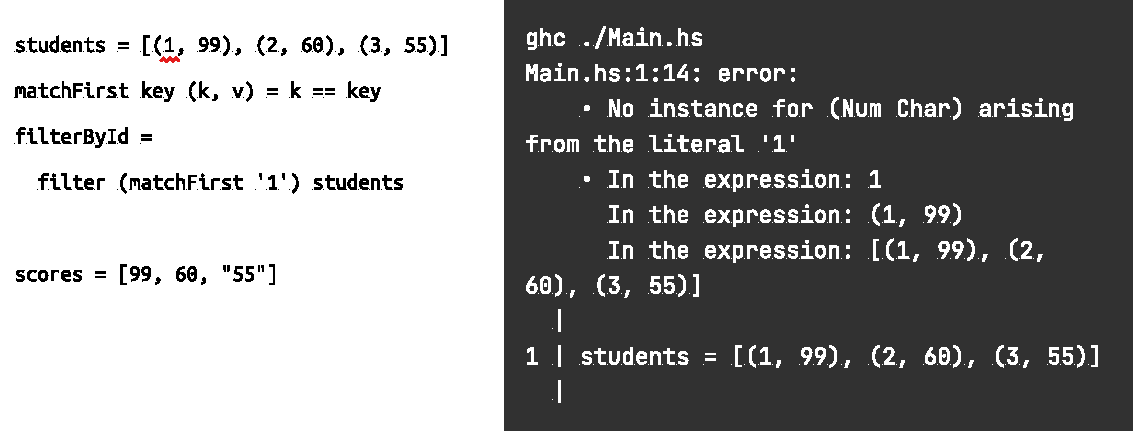
\includegraphics[width=\linewidth]{images/motivation}
        \caption{Inspecting a type error using the Haskell compiler GHC (Glasgow Haskell Compiler)}
        \label{fig:motivation}
    \end{figure}
    To address these challenges of diagnosing and fixing type errors in Haskell, we present a new tool: \textit{Goanna}. Goanna is a Haskell type checker based on Minimal Correct Subset (MCS) enumeration. Compared to traditional type-checking tools, Goanna provides improved type error reporting by giving a comprehensive list of possible causes and suggesting valid fixes for each cause.  Goanna differs from past type debugging systems (as reviewed in Section \ref{sec:related-work}) through its use of Minimal Correction Subsets (MCS), where a single MCS represents a complete set of locations that constitutes a possible cause.

	To further enhance Goanna's support for type-error resolution, we provide optimization strategies (Section~\ref{sub:optimization}) to identify and reduce the unhelpful suggestions, as well as ranking heuristics (Section~\ref{sub:ranking}) to suggest more likely fixes first. Additionally, we provide Goanna-IDE, an interactive debugging front-end designed to efficiently navigate and interpret Goanna's type error diagnosis.

    We conducted empirical studies that evaluated Goanna's accuracy (Section \ref{sub:eval-accuracy}), conciseness (Section \ref{sub:eval-conciseness}), and performance (Section \ref{sub:eval-performacne}). Our evaluation shows that compared to other type-checking tools, Goanna consistently provides accurate error diagnostics and correct fixes in its top suggestions. While Goanna may not consistently provide instantaneous results for real-time feedback, it can deliver on-demand diagnoses when programmers require additional assistance.
    
    The key contributions of this research include:
    \begin{itemize}
        \item A categorization of type errors based on constraint satisfiability
        \item Goanna, a Haskell type checker with improved error reporting based on MCS enumeration and program slicing;
        \item Goanna-IDE, an interactive type error debugging interface for Haskell; 
        \item A collection of heuristics and optimization techniques to enhance MCS-based type error reporting; and
        \item An evaluation of Goanna's accuracy, conciseness, and performance.
    \end{itemize}

  The techniques we used in Goanna, such as MCS enumeration and heuristics for ranking possible causes, are not exclusive to Haskell. Rather, they are applicable to statically typed programming languages in general. We intentionally designed Goanna to use a modular architecture that can be easily extended to support other programming languages with similar typing disciplines.

\section*{A categorization of type errors} \label{sec:category}

To address the complexities in explaining type errors comprehensively, we have identified some common groups of type errors based on how programmers perceive type errors. These include multi-step type errors, multi-witness type errors, and multi-party type errors.


It is crucial to understand that these categories are not mutually exclusive; for example, a multi-witness type error may also be a multi-step type error.

A \textbf{simple type error} simplest type error are the ones involve two fragments of the program that can not agree on a type assignxments. Example like Listing \ref{lst:atomic-error} shows such an error. In the example, x can be inferred as either \texttt{Int} or \texttt{Char} type based on line 1 or line 2. 

\begin{lstlisting}[language=Haskell, caption=The simplest form of type error, label={lst:atomic-error}]
  x :: Int
  x = '3'
\end{lstlisting}

In practice, this kind of type error is very easy to spot. They don't span across different locations, and they do not require mental bookkeeping to trace back to the root cause. When adding more complexity to these errors, they become one of the following groups.


A \textbf{multi-step type error} involves a chain of logical inference steps based on the available evidence of the error. Fig.~\ref{fig:multi-step-example}) illustrates the chains of inference in the assignment of a (Line 1), the equivalence of a (Line 1 and Line 2), the assignment of b (Line 2), and the equivalence of b (Line 2 and Line 3). Removing anyone from the chains will resolve the conflict. Understanding and communicating the interconnections within these chains is crucial to resolving multi-step type errors effectively.

Multi-step type errors occur natually when programs develop layers of indirections or abstractions.

\begin{figure}[htbp]
  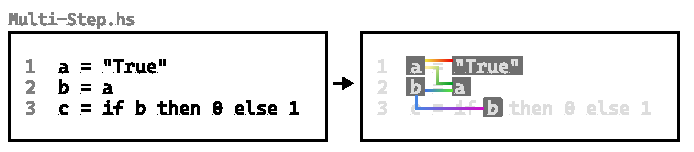
\includegraphics[width=\linewidth]{Multi-Step}
  \caption[This illustration depicts a multi-step type error in Haskell]{
    \label{fig:multi-step-example}
    This illustration depicts a multi-step type error in Haskell. In the program (left panel), the string literal \texttt{"True"} is assigned to the variable \texttt{a} on line 1, followed by the assignment of \texttt{a}'s value to variable \texttt{b} on line 2. Subsequently, on line 3, the program attempts to use \texttt{b} as a boolean condition in an \texttt{if} expression. The error analysis can be visualized as a "chain" of reasoning, represented by the continuous line (right panel), tracing the propagation of the type mismatch through the sequence of assignments and usage. }
\end{figure}

A \textbf{multi-witness type error} involves multiple pieces of evidence supporting the same potential type assignments. For instance, as shown in Fig.~\ref{fig:multi-witness-example}, multiple pieces of evidence (lines 3,4,5) support that \texttt{a} has the type \texttt{Int -> String}. On the other hand, a single piece of evidence (line 2) shows that \texttt{a} has the type \texttt{Int -> Char}.  Clarifying and juxtaposing this discrepancy in witnesses is key to supporting understanding this type of error.

Multi-witness type errors occur when changes to the definition of one fragment of the program, and this fragment is referenced by multiple places. 


\begin{figure}[htbp]
\centering  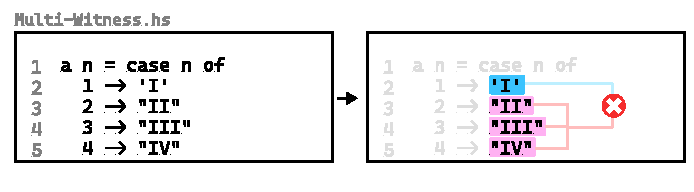
\includegraphics[width=\linewidth]{Multi-Witness}
  \caption[This illustration depicts a multi-witness type error in Haskell]{
    \label{fig:multi-witness-example}
    This figure presents the analysis of a multi-witness type error in Haskell. In the source code (Left), a type conflict arises from the \texttt{case} expression, which could be interpreted as \texttt{Char} based on the value in line 2, or as a \texttt{String} based on the values in lines 3, 4, and 5. The type conflict is graphically illustrated (Right) with \texttt{String} values marked in pink and the \texttt{Char} value in blue. The majority of \texttt{String} value witnesses suggest the lone \texttt{Char} literal \texttt{'I'} on line 2 might be a typographical error. This discrepancy underscores the significance of witness count in identifying the likely error source.}
\end{figure}

A \textbf{multi-party type error} involves several potential type assignments, each supported by distinct evidence.  Fig.~\ref{fig:multi-party-example} presents a typical multi-step type error: the expression \texttt{d} can not be assigned a type because 3 pieces of evidence on line 1 suggest 3 potential types for \texttt{d}. In practice, addressing such errors requires breaking them down into multiple type errors of simpler forms. 

Multi-party type errors are rarer in real life programs, but they can happen when programmers reverse the order of two input arguments. 

\begin{figure}[htbp]
\centering  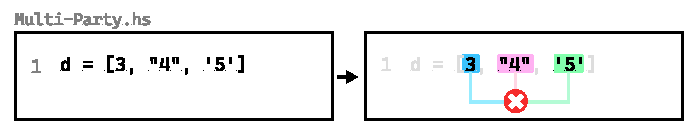
\includegraphics[width=\linewidth]{Multi-Party}
  \caption[This illustration depicts a multi-party type error in Haskell]{
    \label{fig:multi-party-example}
    This figure analyzes a multi-party type error in the source code (Left), where the list \texttt{d} could potentially be typed as \texttt{[Int]}, \texttt{[String]}, or \texttt{[Char]}. The disagreement is visually represented (Right) by three distinct colors, each corresponding to the cause of one of the possible types. This scenario differs from previous examples as resolving the type error requires adjustments at multiple locations within the code, not just a single change.
       }
\end{figure}
  
\section{Related Work} 
    \label{sec:related-work}
    In this section, we survey the corpus of work that Goanna built upon and was inspired by. We first review the work that is built on a theoretical foundation similar to that of Goanna. We then examine studies that share similar aims and offer a debugging experience comparable to Goanna's. Finally, we delve into research on program slicing and discuss how Goanna extends the concept of slicing and distinguishing itself from its predecessors.

    \subsection{MCS enumeration}
	
    MCS enumeration has been extensively studied in the field of error localization across various domains. MCS is used to optimize package management system \cite{Ignatiev2014-nr} and to explain decisions made by machine learning algorithms \cite{Marques-Silva2023-nk}.
    
    
    In the specific context of type error diagnosis and resolution, several related approaches have been explored. It is important to examine the strengths and weaknesses of Goanna in the context of these areas.

    One notable work by Lamraoui et al. introduced a tool \cite{Lamraoui2016-wr} that utilizes the capability of MCS to localize multiple faults and identify software defects using unit tests. Their approach demonstrated the effectiveness of MCS in pinpointing errors within a program. Similarly, Bekkouche et al. conducted a relevant study  \cite{Bekkouche2015-is}  on MCS utilization for locating program errors in while-loop programs. Their findings showed improved efficiency compared to SAT-based approaches. Although showing strength in programming language static analysis, MCS-based fault localization has not been previously applied at the type system level. Goanna distinguishes itself as the first tool to explore this approach within the realm of type error diagnosis and resolution.

    \subsection{Suggesting changes to type errors}
   Lerner et al. proposed Seminal \cite{Lerner2007-mu}, using syntax mutation and binary search to find appropriate syntax changes to program errors. The advantage of Seminal is that it's capable of suggesting direct syntax changes to common mistakes (e.g., mistakingly swapping the order of function arguments). However, it is impossible for Seminal to provide the complete set of all potential fixes. Nor does it guarantee a suggested solution is minimal syntax change.
   
   Counter-factual typing (CFT) \cite{Chen2014-dz,Chen2020-ad} uses a variation-based type system; it is capable of suggesting the correct type for all possible. CFT shares many capabilities with Goanna, CFT is able to suggest multiple-location changes, CFT uses similar ranking heuristics. Goanna is able to produce an in-depth analysis of the ill-type program, such as type error isolation. CFT and Goanna both aim to produce a complete set of potential fixes, Goanna employs a set of effective algorithms to reduce the exponential number of potential fixes without reducing the quality of suggestions. 
   
   SHErrLoc \cite{Zhang2015-xy} uses constraints as the underlying to perform type inference and type error diagnoses. SHErrLoc is able to suggest multiple possible fixes of the type error and rank them based on heuristics. Unlike Goanna's approach of using a general-purpose constraint language, SHErrLoc relies on GHC's internal constraints and then translates them into SCL (a custom-made constraint language). On the technical side, this approach relies heavily on modification of the compiler and does not remain reliable with later GHCs. Most importantly, there is no way to interact directly with the solver. This renders the kind of constraint manipulation in Goanna and SHErrLoc impossible. Goanna is able to perform type reconstruction for ill-typed programs, that is, finding the most concrete types for all expressions for each potential solution using the Maximal Satisfiable Subsets. SHErrLoc focuses on finding the locations only.


\subsection{Type Error Slicing}

Type error slicing \cite{Haack2004-fr} is a technique to identify all necessary locations of a type error that is necessary for programmers to diagnose the root cause. It has been studied in many studies ever since \cite{Tip2001-qn, Heeren2003-kd}. These studies all use Minimal Unsatisfiable Subset (MUS) to ensure the \textit{completeness} and \textit{minimality}. The drawback of type error slicing is that it often produces too many locations.  Chameleon \cite{Stuckey2003-pz,Fu2021-xd} improved type error slicing by allowing programmers to interactively show the partial MUS by choosing their own assumptions. Compared to these tools that base their analysis on a single MUS, Goanna effectively utilizes all possible MUSes. This allows Goanna to enhance its suggestions based on the improved knowledge of the underlying type of error. For example, it uses the number of MUSes a location appears in to rank how likely the location is part of the root cause. This is not possible with a single MUS.  


\section{Goanna-IDE Walkthrough} \label{walkthrough}
In this section we  demonstrate Goanna's features using some real world examples. To showcase the debugging features,  we developed Goanna-IDE, a type error debugging interface for Haskell. Goanna-IDE is designed around the pitfalls of common typecheckers and the different categories of type errors. It make extensive use of Goanna's type error diagnosis through visualization and interactivity. Goanna-IDE provides comprehensive diagnostic error messages for type errors in Haskell and allows programmers to interactively explore their options. An online demo of Goanna-IDE is available for evaluation at \cite{Fu2023-bo}. Goanna-IDE includes a file explorer, a text editor, and a debugging panel. Goanna-IDE provides the following features when type errors are encountered:

    \begin{itemize}
        \item Thoroughly detect all type errors within the codebase and allow users to inspect each type error individually via the debugging panel.
        \item Indicate the most likely causes by star indicators.
        \item Show necessary type hints in the editor panel to help reason about each possible cause.
        \item Allow users to trace type errors across multiple files.
    \end{itemize}

    \subsection{Examples of Diagnosing Type Errors with Goanna-IDE}

    For the type error in the motivating example, Goanna shows 6 possible causes of the error (see top right corner of Fig.~\ref{fig:goanna-example-1}). When focussing on the cause suggested by GHC, instead of highlighting only the literal \texttt{1}, Goanna reports all 3 literals that needed to be changed all at once if the programmer chooses to address this cause. In addition, Goanna also indicates that these integer literals need to be changed to \texttt{Char} type using the inlay type hints on line 1, largely narrowing down the potential ideal fixes. 
    

    \begin{figure}[ht!]
        \centering
        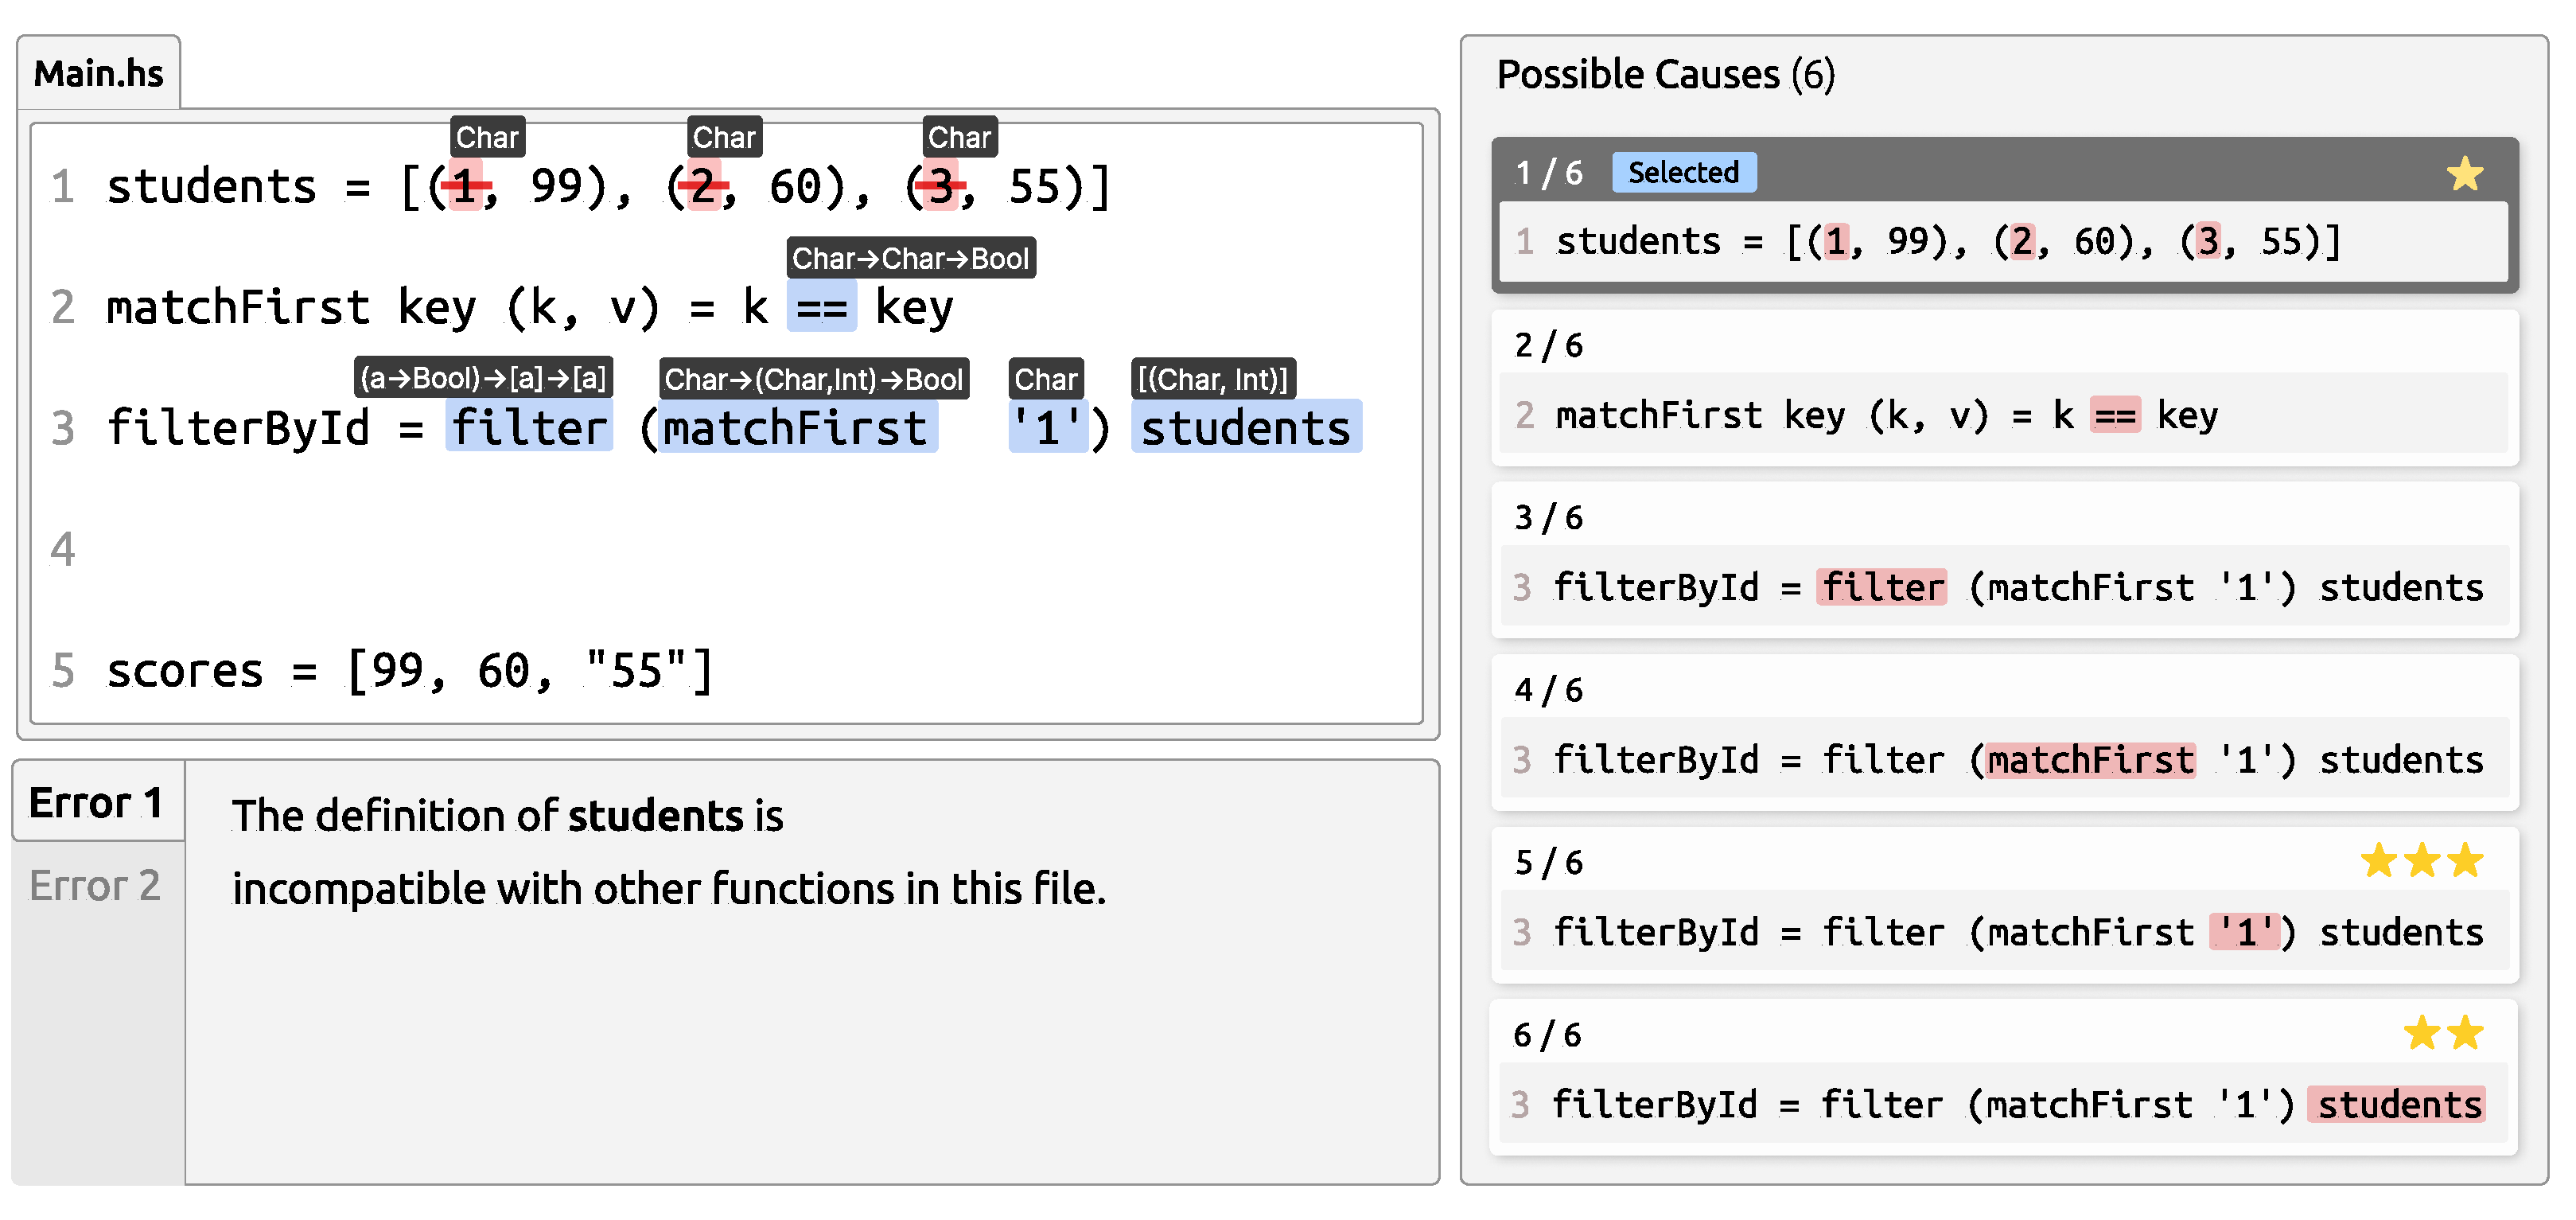
\includegraphics[width=\linewidth]{images/Goanna-Example-1}
        \caption[Goanna's showing possible causes of a type error (1)]{\textbf{Goanna's error diagnosis} Goanna shows that to fix the type error, the literals \texttt{1}, \texttt{2}, and \texttt{3} on line 1 need to be changed to Char type.}
        \label{fig:goanna-example-1}
    \end{figure}


    Note that the cause suggested by GHC is only one of the possibilities identified by Goanna. In fact, Goanna suggests that there are more likely fixes, indicated by the star symbols. The most likely fix, based on Goanna's cause heuristics (Section \ref{sub:ranking}), is the \texttt{Char} literal \texttt{'1'} on line 5, indicated by the 3 stars (Fig.~\ref{fig:goanna-example-1}).
    
    
    By clicking on the most likely cause, Goanna shows different highlights in the editor (e.g., see Fig.~\ref{fig:goanna-example-2}). Goanna reports the error is caused by the literal \texttt{'1'} and suggests changing to an integer. All the type hints are adjusted based on our new assumption. Goanna ranks all possible causes using a series of heuristics. In this case, the preference is largely influenced by how many locations are required to change to fix the error. 
    
    \begin{figure}[ht!]
        \centering
        \includegraphics[width=\linewidth]{images/goanna-example-2}
        \caption[Goanna's showing possible causes of a type error (2)]{\textbf{Goanna's error diagnosis.} Goanna shows that the type error can be fixed by changing the literal $'1'$ on line 3, which needs an \texttt{Int} type. This, according to Goanna, is the most likely cause of the type error.}
        \label{fig:goanna-example-2}
    \end{figure}


    \subsection{Identifying all type errors} \label{sub:all-errors}
    
    A key feature of Goanna is its ability to detect all type errors in the code thanks to its MCS enumeration (Subsection \ref{sub:enumeration}). This is not always the case with other tools, such as GHC, which may only report a subset of the errors present in the code or stop at the first error they encounter. Goanna, however, always thoroughly identifies all type errors in the codebase. In the example of Fig.~\ref{fig:goanna-example-1} and Fig.~\ref{fig:goanna-example-2}, Goanna discovered the two errors included in the file. Clicking on the error selector on the bottom-left will change the content of the debugging panel and text editor highlights to reflect the cause of a different error (Fig.~\ref{fig:multi-error}). 

    \begin{figure}[ht!]
        \centering
        \includegraphics[width=\linewidth]{images/goanna-multi-error}
        \caption[Selecting a different error in Goanna]{\textbf{Selecting a different error in Goanna.} Selecting a different error using Goanna's error selector. The debugging panel will show potential cause locations for the selected error. The highlights and type hints in the editor panel will focus on the selected error.}
        \label{fig:multi-error}
    \end{figure}



    \subsection{Type error grouping}  \label{sub:group}
    In addition to reporting multiple errors, Goanna also groups together type errors that might be treated as separate by other tools. Goanna uses a novel approach (section \ref{sub:grouping}) to ensure that type errors that are intuitively connected are grouped together. This means that Goanna does not overwhelm the programmer with an excessive number of redundant type errors. Instead, the programmer is presented with a concise list of errors that all can be assessed separately.

    \begin{figure}[ht]
        \centering
        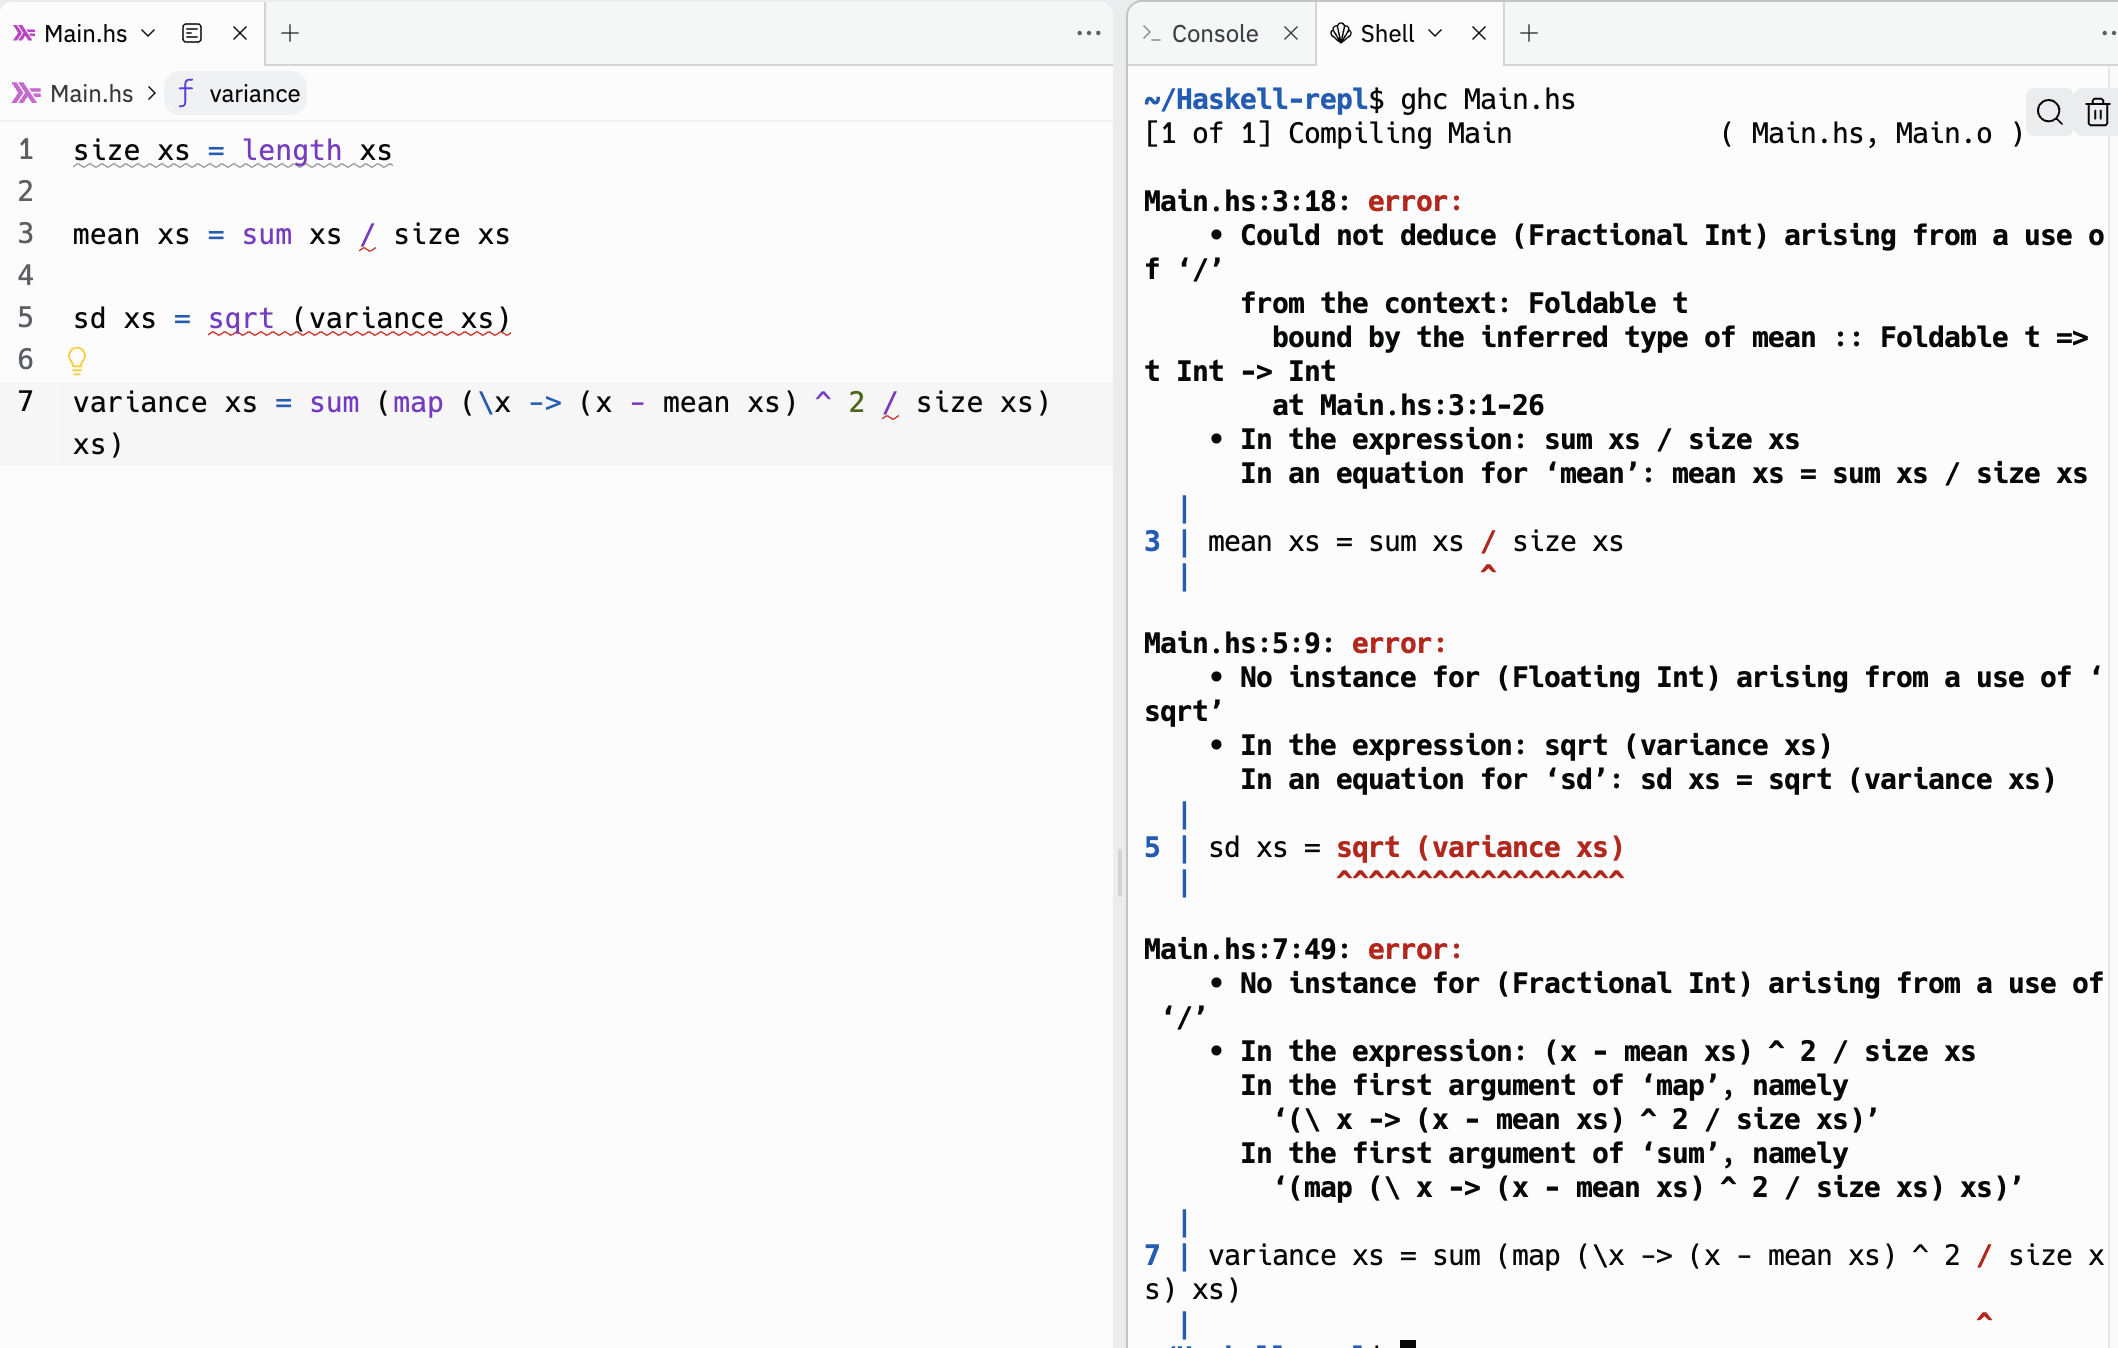
\includegraphics[width=\linewidth]{images/variance-ghc}
        \caption[Inspecting a defective Haskell Program in relation to the error messages output by the standard GHC compiler]{\textbf{Inspecting a defective Haskell Program (left) in relation to the error messages output by the standard GHC compiler (right)} -- 3 separate type errors are reported.  The editor (VS Code is used here) underlines the error locations reported in the messages, but all other contextual information must be understood from the error text.}
        \label{fig:grouping-ghc}
    \end{figure}
    
        \begin{figure}[ht!]
        \centering
        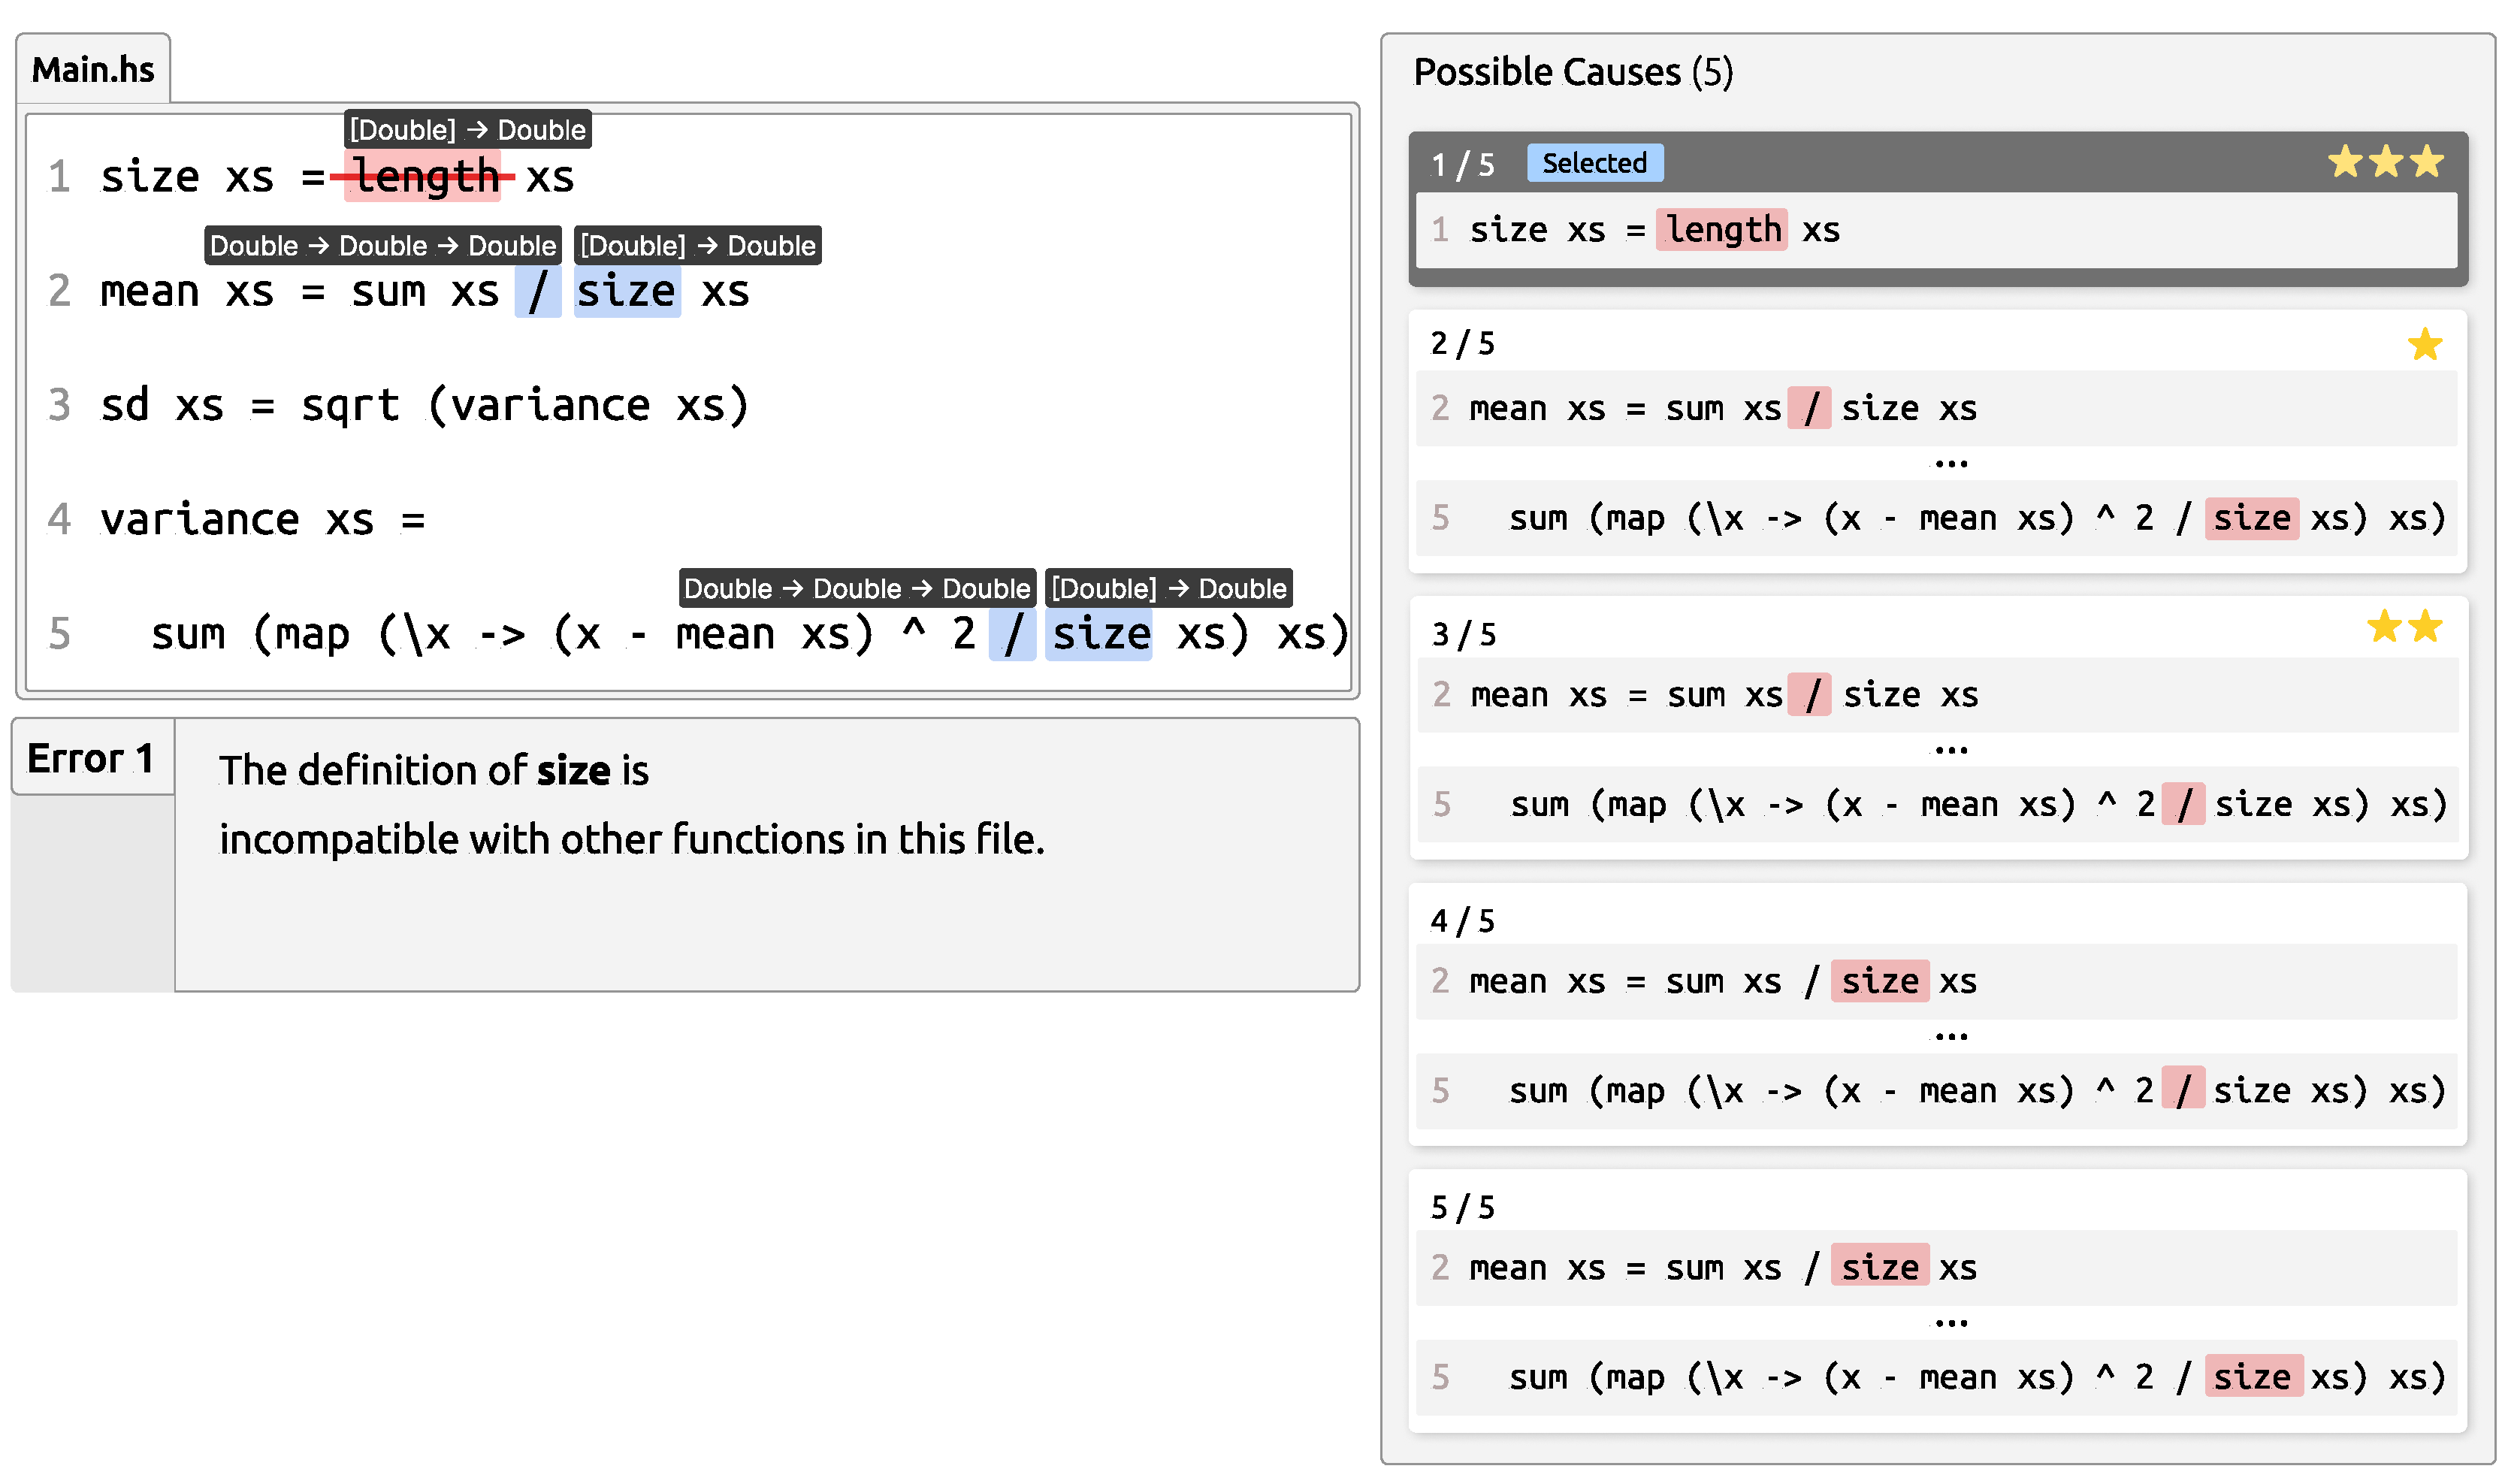
\includegraphics[width=\linewidth]{images/Goanna-Error-Grouping}
        \caption[Goanna's Error Grouping]{\textbf{Goanna's Error Grouping.} This error, although its potential offending parts appear in many declarations, is possible to fix in one place, i.e., by changing the definition of the \texttt{size} function on line 1. Therefore, Goanna reports it as a single error.}
        \label{fig:grouping-goanna}
    \end{figure}

    For instance, in Fig.~\ref{fig:grouping-ghc}, the functions \texttt{variance} and \texttt{mean} expect the final type of \texttt{size} to be a fractional value. However, the definition of \texttt{size} results in an integral value, which creates a conflict. While GHC shows three separate type errors, Goanna groups these interconnected errors into a single entity, as shown in Fig.~\ref{fig:grouping-goanna}. These errors can be addressed collectively, thereby improving the efficiency of the programmer.

    \subsection{Discovering Potential Causes} \label{sub:suggesting}
    When a type error arises, Goanna-IDE shows a list of possible causes in the debugging panel. Each possible cause consists of one or more locations in the code that require modification to rectify the type error. Clicking on a possible cause activates it. The locations are highlighted in the text editor, as well as inlay type hints suggesting the suitable type expected for that code slice. In the debugging panel, the activated cause is outlined with a red icon, while others are marked with a blue icon. 

    The causes identified by Goanna are comprehensive. Goanna will take into account potential causes in expressions, pattern matchings, type annotations, and type class constraints. Consequently, programmers will generally find the real cause by exploring Goanna's diagnosis. Unlike most Hindley-Milner~\cite{Damas1982-zw} based type inference, Goanna does not show a bias towards the unification order, thereby avoiding the left-to-right bias \cite{Chen2014-ev}. 
    
    Note that Goanna's fixes are sufficient to resolve the type error. Traditional tools often reveal a set of partial locations of a type error, leaving programmers to realize later that additional adjustments are needed for a complete resolution. Goanna, however, offers fixes that encompass a complete set of changes necessary for a resolution.


    \subsection{Assessing Likelihood of Causes} \label{sub:conciseness}
    One challenge of Goanna's ``find all causes" approach is the number of ways an error can occur can sometimes become too large to be useful in practice. Goanna employs multiple techniques to intelligently sieve the list. For the remaining list, Goanna employs a few heuristics to rank their likelihood and inform programmers which causes they consider first. 
    Goanna-IDE uses a star-based rating system to signal the ``likelihood'' of each cause. 3 stars indicating the most likely cause, 2 stars and 1 star follows. 

    \subsection{Type Hints}\label{subset:type-hints}
    In addition to suggesting which part causes that type error, Goanna-IDE explains why this is inferred by using in-situ type hints on necessary terms. The type hints are displayed as inlay decorations on top of respective fragments of source code. These type hints provide enough information for programmers to understand the type inference, and Goanna will leave out the terms that are irrelevant to the type error. Goanna's type hints are also dynamic to the selected cause. Programmers can observe how the inferred type of each term changes by changing the selected cause. Many modern programming tools use inlay type hints to support understanding, such as   Haskell Language Server~\cite{HLS-Developers2023-ot},  most often, these tools will display all type hints or none. Unlike in Goanna, these tools do not provide alternative sets of type hints for programmers to compare.
    
    \subsection{Cross-module type error debugging}\label{subsec:cross-module-type-error-debugging}
    When encountering a type error spanning across multiple modules, Goanna-IDE will group the potential causes indicated by their module and declaration block. Clicking on any possible cause location will focus the editor on the corresponding module (Fig.~\ref{fig:goanna-cross-module}). Goanna is the first tool to introduce cross-module type debugging. The way Goanna presents cross-module type errors is analogous to how run-time errors are presented in most programming languages. When encountering a run-time error, most programming environments show a call stack containing multiple file paths, and programmers can choose which file to start investigating. Often, programmers choose to start from the file authored by themselves instead of library files. Goanna uses this mental model to group potential locations that cause a type error by module and definition blocks. 
    
    \begin{figure}[ht!]
        \centering
        \includegraphics[width=\linewidth]{images/goanna-cross-module}
        \caption[Debugging a cross-module error in Goanna]{\textbf{Debugging a cross-module error in Goanna.} In this error, potential defects may appear in either module \texttt{A} and \texttt{B}. Goanna suggests 3 potential causes and fixes: 1) Change the type annotation of \texttt{x} to \texttt{[Maybe Int]} (Top). 2) Change the y variable on line 4 of module \texttt{A} to an instance of \texttt{Int}. 3) Change both the elements in the list literal in module \texttt{B} (Bottom), hence affecting the type of \texttt{y}. Clicking on each potential cause in the debugging panel results in different highlights and type hints in the editor panel.}
        \label{fig:goanna-cross-module}
    \end{figure}


    \section{Goanna Implementation} \label{sec:implementation}
    Goanna comprises 3 phases: constraint generation, MCS enumeration, and post-analysis. In the constraint generation phase, Goanna walks the abstract syntax tree and collects constraints. In the MCS enumeration phase, Goanna enumerates through all MCSes. Lastly, in the post-analysis phase, Goanna applies multiple optimization techniques to reduce the number of MCSes, group MCSes by common properties, and sort them based on heuristics.

    Goanna supports a wide and growing range of the Haskell 2010 language syntax \cite{Simon_Marlow2010-lg}. At the time of writing, fully supported features include module import/export, qualified imports, import hiding, do notation, algebraic data types, newtypes, type synonyms, type classes, operator sectioning, and range expression. Only operating in the type level, Goanna automatically support the language extensions that are not type related (RecordWildcard), and those do not extend the rules of the underlying type system (InstanceSigs). Overall Goanna support the most highly used type level extensions in Haskell and the range of supported feature is continue growing.  A detailed and updated feature coverage list can be found in \cite{Fu2023-rp}.

    \subsection{Constraint Generation} \label{sub:translation}
    Goanna uses the abstract syntax tree of the original Haskell program and translates it into a constraint program by modeling how types are defined and used. Goanna does not restrict which constraint language and solver should be used. The only requirement is that Goanna needs to be able to assert whether a subset of the constraints is still feasible by calling a provided \texttt{solve} function during the MCS enumeration phase. In our implementation, we generate portable Prolog predicates \cite{Wielemaker2011-sr}. The \texttt{solve} function executes a predefined predicate \texttt{type\_check/0} that tests all the generated predicates. We used standard Prolog notation \texttt{name/arity} here when referring to Prolog predicates, as a Prolog predicate is identified by the combination of both attributes. 

    
    For a simplified Haskell syntax shown in Fig.~\ref{fig:translation}.A, we generate a list of Prolog predicates in the language shown in Fig.~\ref{fig:translation}.B. We use 3 auxiliary functions during the constraint translation process (Fig.~\ref{fig:translation}.C) to generate Prolog variables for future unification. \texttt{fresh} makes a unique unbound Prolog variable. \texttt{var} takes a Haskell identifier name and returns a Prolog variable. Naively, this can be done by turning it to uppercase. \texttt{atom} takes a Haskell type constant/constructor name and returns a Prolog atom. Naively, this can be achieved by turning it into lowercase. We keep track of local variable names in a list $\Gamma$ containing Haskell variable names. A global variable $\mathcal{P}$ is defined to store the list of predicates being generated. To clarify, all \textcolor{blue}{parsed Haskell syntax} are in blue. All \textcolor{red}{generated Prolog syntax} are in red. 
    
    Two sets of generation rules apply to different syntax nodes and output Prolog source code. Predicate generation rules (Fig.~\ref{fig:translation}.D) take Haskell declarations as input and output Prolog predicates. For example, a Haskell function \texttt{f = 2}, Goanna may generate a predicate \texttt{\textcolor{red}{f(V, \_) <- V = int.}}
    
    Constraint generation rules (Fig.~\ref{fig:translation}.E) take a Haskell expression node or type node and a Prolog variable \texttt{V} as input and output a list of Prolog terms. These terms attempt to unify the inferred type of such node to the provided Prolog variable \texttt{V}.
    
    \begin{figure}[ht!]
        \centering
        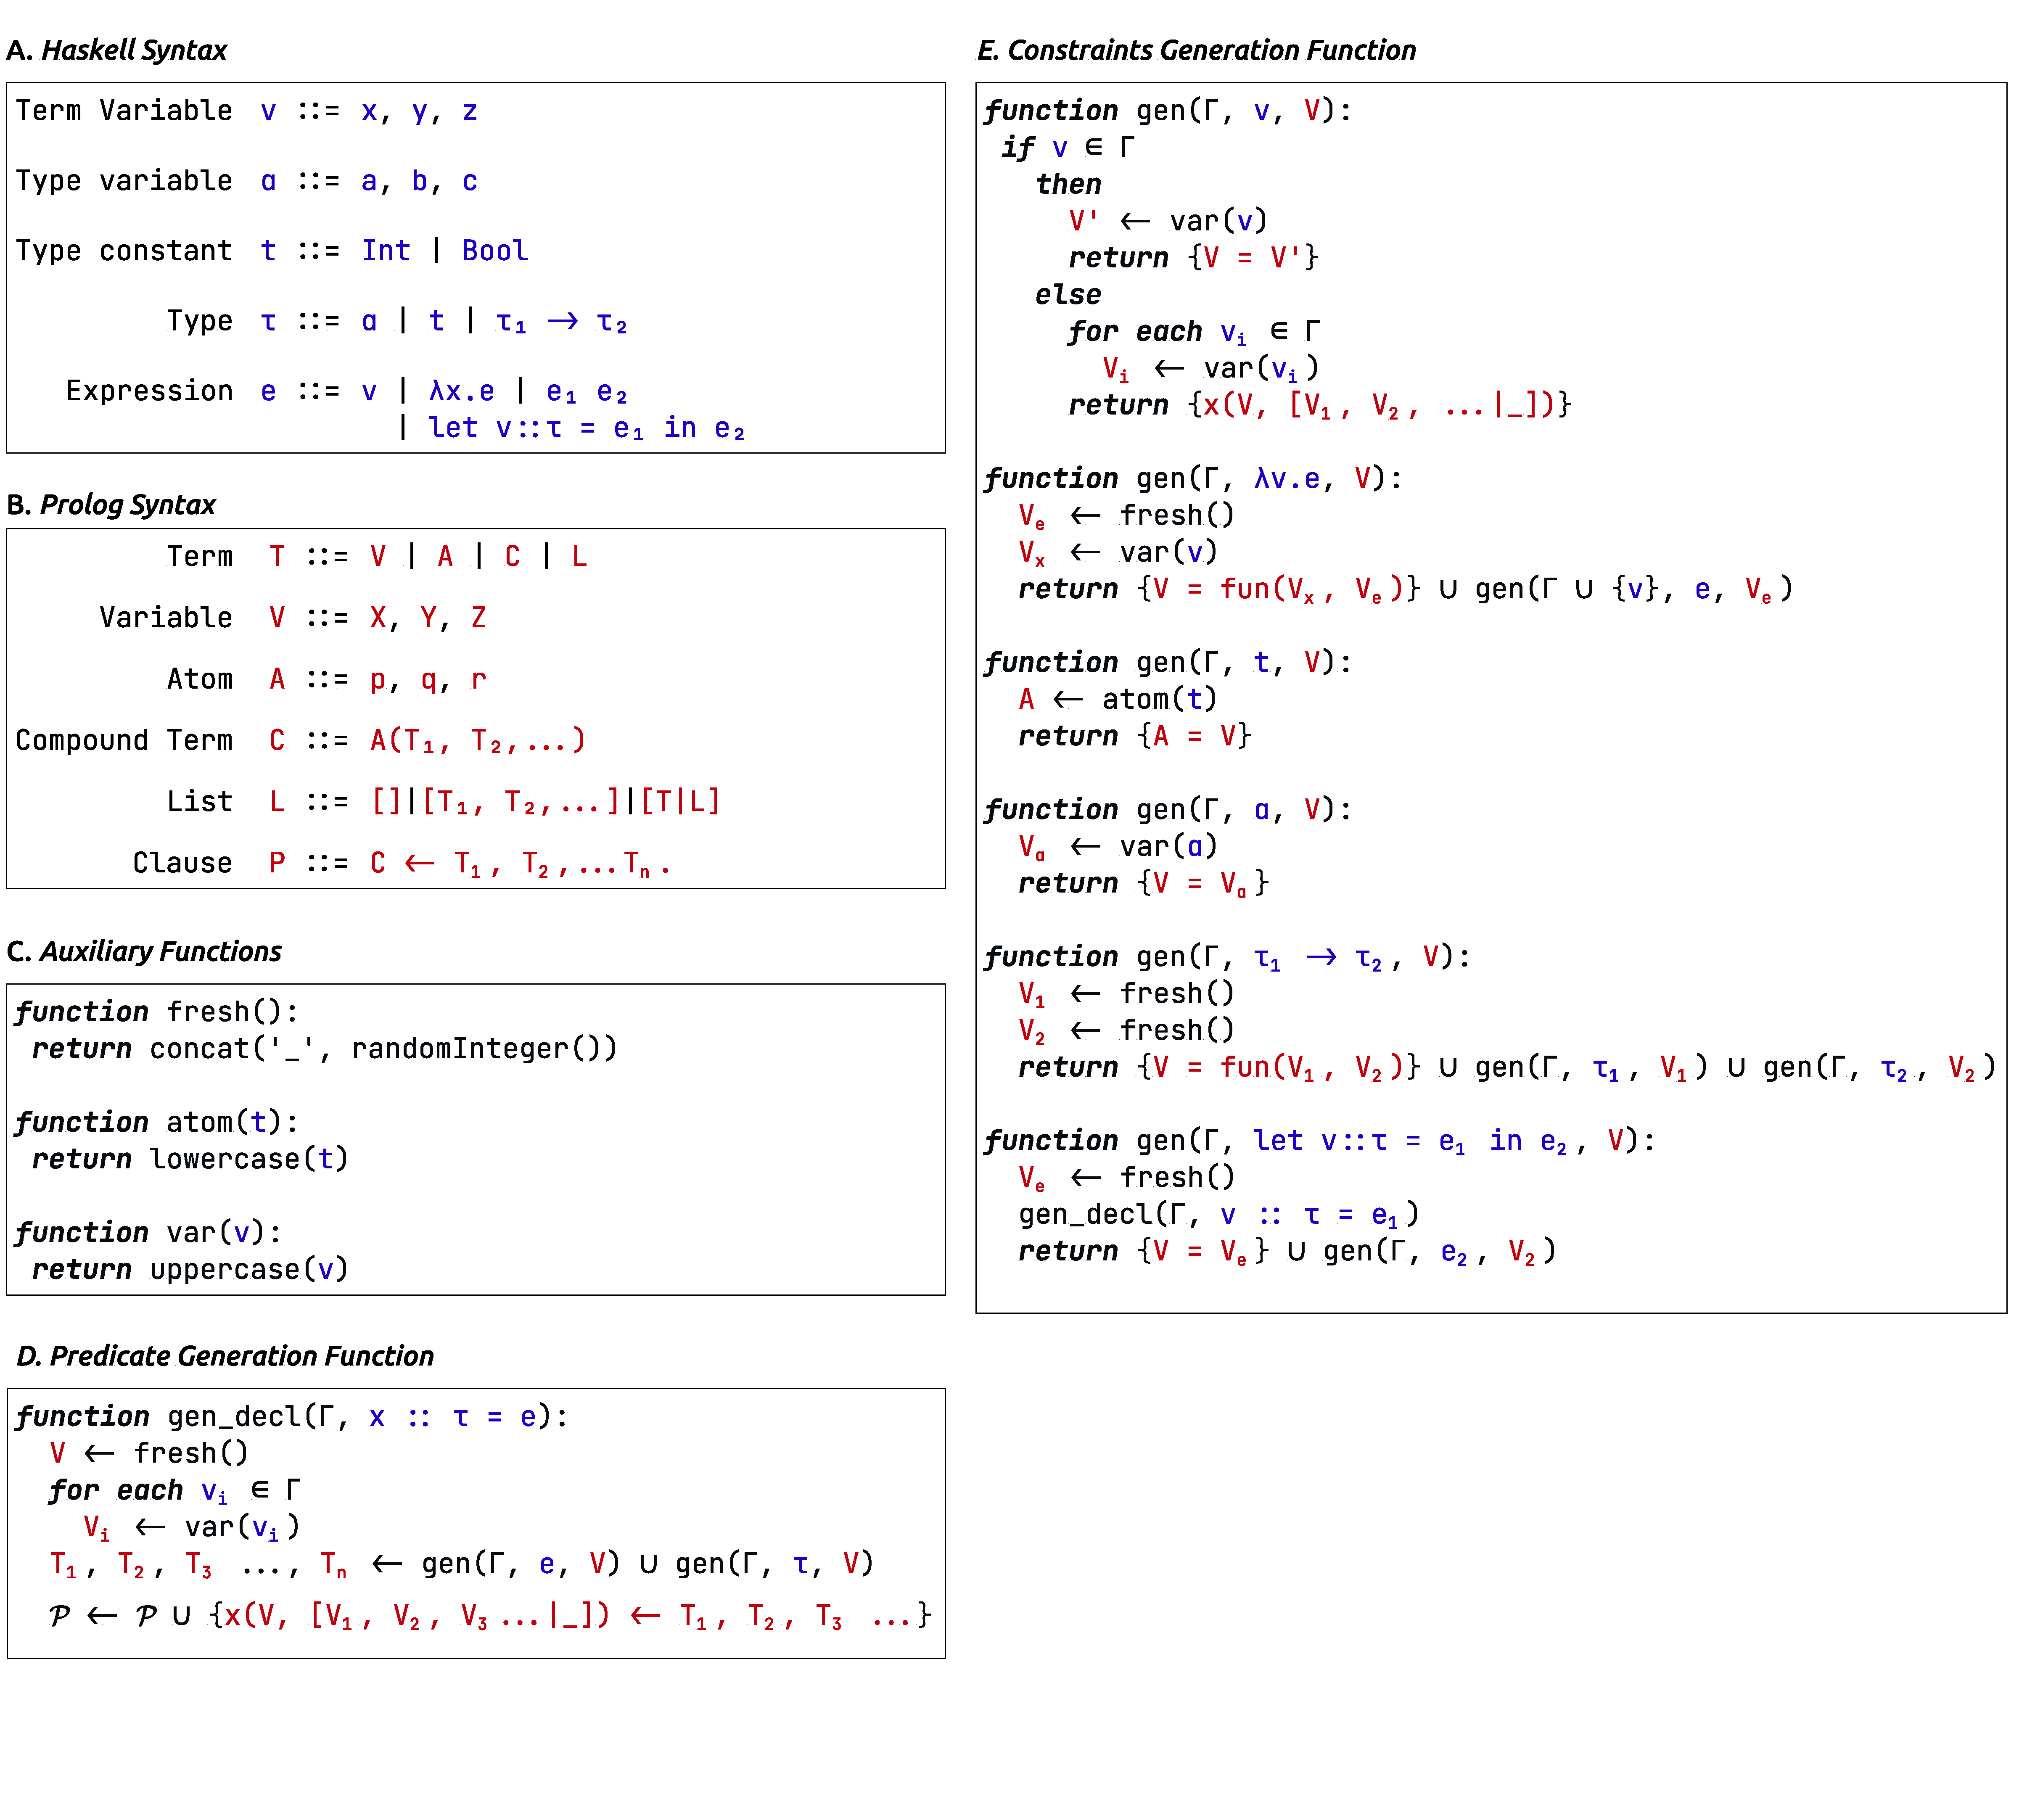
\includegraphics[width=\linewidth,trim={0 6cm 0 0},clip]{images/Generation}
        \caption{Goanna's Constraint Translation Rules (Simplified)} 
        \label{fig:translation}
    \end{figure}
    
  
    An example of such translation can be found in Fig.~\ref{fig:translation-example}. In the Haskell program (Fig.~\ref{fig:translation-example}.A), 2 functions are declared: \texttt{f} and \texttt{g}. This will generate two corresponding Prolog predicates \texttt{f/2} and \texttt{g/2}. In the actual implementation of Goanna, the generated predicates would be \texttt{f/6} and \texttt{g/6}. The extra arguments are added to perform various tasks involving syncing state, such as breaking recursive calls and collecting type class constraints. In a predefined predicate \texttt{type\_check/0}, the subgoals \texttt{f(\_,\_)} and \texttt{g(\_,\_)} are added. Executing the top-level goal \texttt{type\_check} in a Prolog environment will get a result of \texttt{false}.
    
  \begin{figure}[htb]
        \centering
    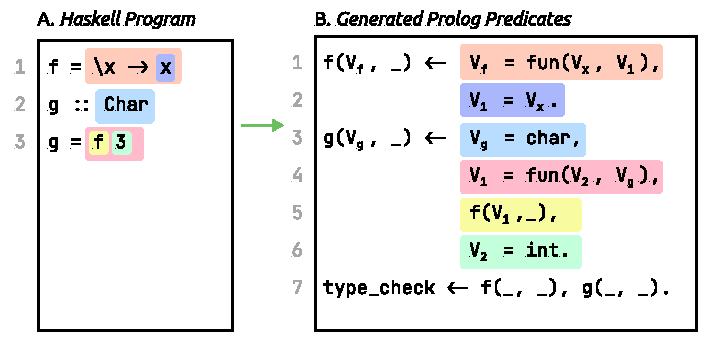
\includegraphics[width=0.7\linewidth]{images/Translation-Example}
        \caption[An example of Goanna constraint generation]{\textbf{An example of Goanna constraint generation.} For the Haskell functions \texttt{f} and \texttt{g}, Goanna generates the predicates \texttt{f/2} and \texttt{g/2}. Each subgoal of \texttt{f/2} and \texttt{g/2} is generated from a corresponding part of the Haskell program. In a predefined predicate \texttt{type\_check/0}, the subgoals \texttt{f(\_,\_)} and \texttt{g(\_,\_)} are added. Running the goal \texttt{type\_check} will return whether the program is well-typed. In this particular example, this will return \texttt{false}. We used standard Prolog notation \texttt{name/arity} here when referring to Prolog predicates, as a Prolog predicate is identified by the combination of both attribute. 
}
        \label{fig:translation-example}
    \end{figure}
    

    \subsection{MCS enumeration} \label{sub:enumeration}
    After the constraint generation phase, Goanna obtains a list of constraints derived from the source code and is able to query the feasibility of any subset of the constraint system by calling the \texttt{solve} function. Goanna uses the MARCO algorithm \cite{Liffiton2016-xi} to efficiently enumerate all MCSes. The benefit of the exhaustive search of MCSes is that we acquire all the MUSes as well largely due to the hitting set duality, and we acquire all the MSSes due to they are complementary relation to MCSes.  To clarify, We refer to the complete set of constraints as a constraint system $C$. When we use the word subset without specifying the corresponding superset, it can be inferred as the subset of the constraint system $C$. We list these subsets obtained from MCS enumeration and give their type-theoretic interpretation. 
    
        
    – A minimal unsatisfiable subset (MUS) $M$ of a constraint system $C$ is a subset $M \subseteq C$ such that $M$ is unsatisfiable and $ \forall{c} \in M : M \setminus \{c\}$ is satisfiable. An MUS can be seen as a minimal explanation of the constraint system’s infeasibility. MUSes have been used extensively, mostly in combination with programming slicing, as a means to explain type errors. A MUS of type system constraints reasoning chain connecting all evidence from one location of the conflict to another. Goanna uses the set of all MUSes to group related type errors.

    – A minimal correction set (MCS) $M$ of a constraint system $C$ is a subset $M \subseteq C$ such that $C \setminus M$ is satisfiable and $\forall{S} \subset M : C \setminus S$ is unsatisfiable. MCSes are so named due to the fact that their removal from $C$ can be seen to “correct” the infeasibility. In an ill-typed program, an MCS $C$ can be seen as the ``cause" of a type error; the removal of C will result in the system being well-typed. Goanna uses MCS to represent potential causes of a type error. Each MCS contains the set of locations that need to be changed to fully resolve the type error.
    
  – A maximal satisfiable subset (MSS) $M$ of a constraint system $C$ is a subset $M \subseteq C$ such that M is satisfiable and $\forall{c}\ in\ C \setminus M:M\cup\{c\}$ is unsatisfiable. The definition of an MSS is symmetric to that of a MUS, with “satisfiable” and “unsatisfiable” swapped along with maximal for minimal. MCS and MSS are the complement sets of one another. In an ill-typed program, an MSS $M$ can be seen as the resulting typing environment if a type error is fixed by excluding the MCS $C - M$. Goanna uses an MSS to provide type hints for the program even when it is ill-typed.
  
 
     \begin{figure}[ht!]
        \centering
        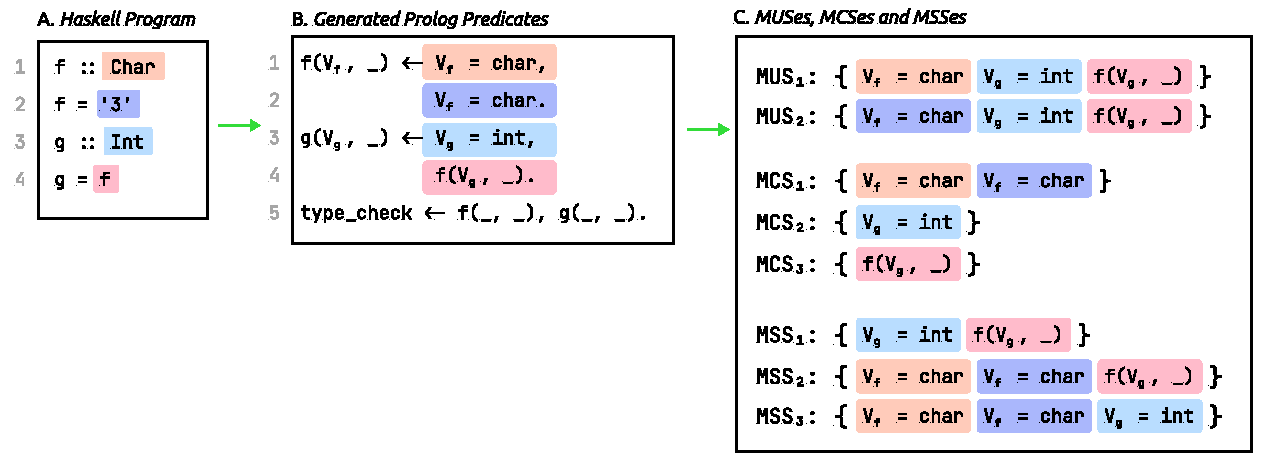
\includegraphics[width=\linewidth]{images/Enumeration-Example}
        \caption[An example of Goanna MCS Enumeration]{\textbf{An example of Goanna MCS Enumeration.} From the set of constraints (B) generated from the Haskell program(A), Goanna obtained 2 MUSes, 3 MCSes, and 3 MSSes. }
        \label{fig:enumeration-example}
    \end{figure}
    
   For the example in Fig.~\ref{fig:enumeration-example}, Goanna's MCS enumeration system identifies 2 MUSes, 3 MCSes, and 3 MSSes. Following the 3 MCSes, Goanna reports 3 potential causes of the type error: the type annotation and function definition in \texttt{f} (from $MCS_1$), the type annotation alone in \texttt{g} (from $MCS_2$), and the function definition alone in \texttt{g} (from $MCS_3$). 

 
\subsection{Type Error Grouping} \label{sub:grouping}

Sometimes, it is insightful to inform programmers type inconsistencies are related to each other (caused by the same violation of typing rules) or isolated instances. To achieve this, Goanna introduce a novel feature called type error isolation. When knowing the all the MUSes, Goanna is able to analyse how many isolated type errors are there and what are the locations involved in each type error. The algorithm of performing type error isolation is as such:


	Let $U$ denote the set of all Minimal Unsatisfiable Subsets (MUSes) and $C$ the set of all Minimal Correction Sets (MCSes). We define an undirected graph $G$, where each vertex in $G$ corresponds to a minimal unsatisfiable subset $u_i \in U$, and the edges of $G$ connect pairs of MUSes $u_i$ and $u_j \in U$ if their intersection is non-empty. The set of all connected components $D$ in $G$ represents the set of all type errors. For each $d_i \in D$, let $l_i = \bigcup v_i$, where $v_i$ is the set of vertices in $d_i$. $l_i$ is the set of all constraints local to this type error. Define $C_i = \{ x \mid \forall c \in C, x = c \cap l_i \}$ as the set of all MCSes that are local to this type error.


    This can be intuitively thought of as follows: two type errors can be grouped together if they cannot be fixed independently through modifying a minimal set of locations for each. For instance, Fig.~\ref{fig:grouping-example}.A shows one connected type error, where there are two fixes available: change \texttt{0} on line 1 to a Boolean type, change the type annotation on line 3 to a \texttt{Num} instance, or change the assignment of \texttt{y} to a different expression. Choosing either one will result in both \texttt{x} and \texttt{y} being inferred to have a valid type.
    


   \begin{figure}[ht!]
        \centering
        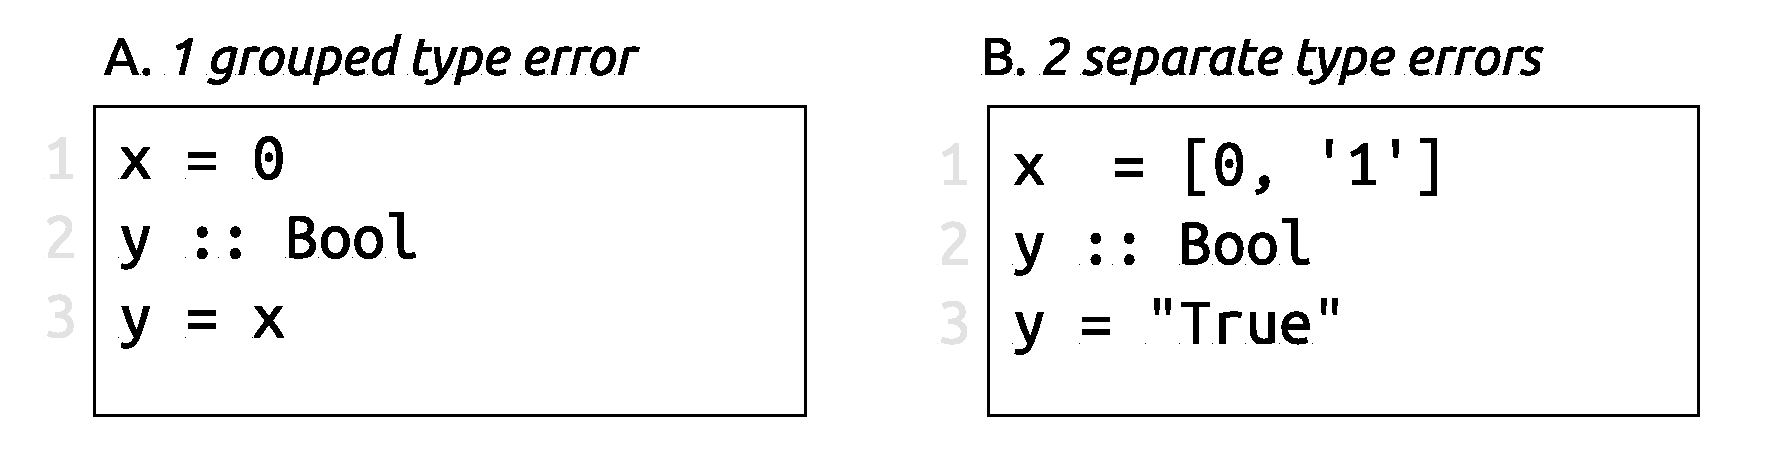
\includegraphics[width=0.8\linewidth]{images/Grouping-Example}
        \caption[Goanna's type error grouping]{\textbf{Goanna's type error grouping.} The ill-typed program on the left contains a single type error, because it can be fixed by a minimal set of syntax changes. For example, fixing it by changing the literal \texttt{0} on line 1 to \texttt{True} or \texttt{False}. This edit contains a single location, so there exists no smaller edit that can fix \texttt{x} or \texttt{y} alone. The program on the right contains two type errors because \texttt{x} or \texttt{y} can be fixed separately. For example change \texttt{0} to \texttt{'0'} on line 1 fix \texttt{x} alone. }
        \label{fig:grouping-example}
    \end{figure}



    However, in Fig.~\ref{fig:grouping-example}.B, although the ill-typed fragment is in a single function, we can fix the argument, either \texttt{0} to \texttt{'0'} or \texttt{'1'} to \texttt{1} to eliminate part of the type error. The same goes for the function's result type \texttt{x}. In this case, there are two separate type errors that should not be grouped.

	In practice, type error grouping provides a sense of the ``effective area" of a type error. Programmers are commonly bewildered by the fact that changing one place of the program causes an error in a seemingly unrelated area. When refactoring a known correct program, a programmer can change the definition of one variable, and Goanna will show all the locations that require further changes. This works because all the further changes belong to the same type error, because a single syntax change -- reverting the initial changes -- will result in the program being well-typed once more.
	
	More specifically, to Goanna, type error grouping provides an effective means to reduce the number of causes. In an ill-typed program with $m$ errors, each having $n$ potential causes, will result in $nm$ total causes. Dividing these causes into separate errors that align correctly with intuition is the most important technique to enhance Goanna's error reporting.

    \subsection{Cause Ranking} \label{sub:ranking}
     In Goanna-IDE, when a list of potential causes is on display, Goanna-IDE also shows the top 3 ``likely" causes according to the ranking heuristics. This is very helpful because programmers will have a starting point for the investigation. We provide a set of efficient heuristics for ranking suggestions. 

    \paragraph{Number of Error Locations.}
    Causes comprising fewer locations are prioritized and presented earlier in the list. For instance:
   \begin{figure}[ht!]
        \centering
        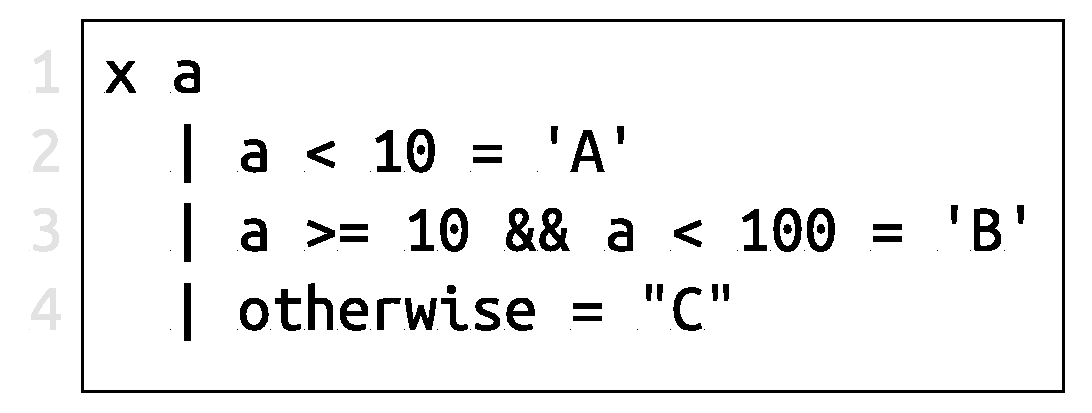
\includegraphics[width=0.5\linewidth]{images/Loc-Count}
        \caption[Goanna prefers causes with fewer error locations]{\textbf{Goanna prefers causes with fewer error locations.} In this ill-typed program, Goanna chooses to give the cause \texttt{"C"} on line 4 a higher likelihood because it contains a single location. The other cause contains 2. }
        \label{fig:loc-count}
    \end{figure}

    In the example in Fig.~\ref{fig:loc-count}, there exist two possible fixes: 1) Changing \texttt{'A'} and \texttt{'B'} to the string type, and 2) changing \texttt{"C"} to the \texttt{Char} type. As the latter fix affects only 1 location (as opposed to 2 in the former), it is assigned a higher ranking and appears earlier in the list.

    \paragraph{Change specificity.}
	Another useful heuristic is to encourage the cause whose fix will result in every surrounding term to be as concrete as possible.
	
	
   \begin{figure}[ht!]
        \centering
        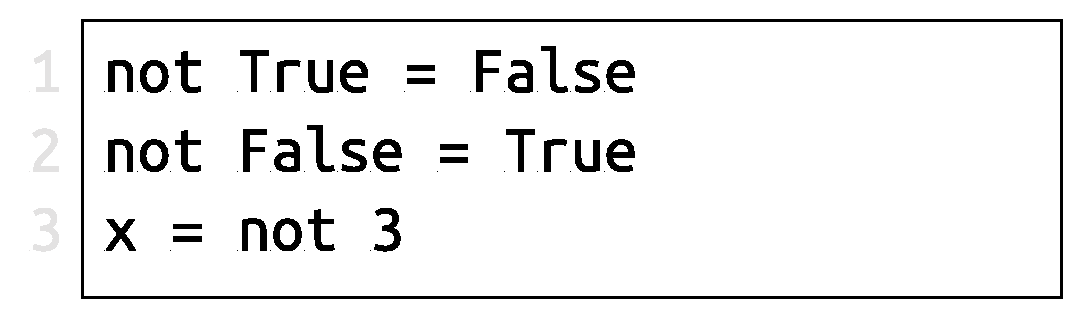
\includegraphics[width=0.5\linewidth]{images/Specificity}
        \caption[Goanna prioritize causes whose resolutions lead to more concrete type assignments]{\textbf{Goanna prioritize causes whose resolutions lead to more concrete type assignments.} In this example, change \texttt{3} will result in \texttt{x} to have type \texttt{Bool}. Alternatively, \texttt{x}'s type will be unknown after changing \texttt{not} on line 3. Goanna prefers the former.} 
        \label{fig:specificity}
    \end{figure}

    In the example in Fig.~\ref{fig:specificity}, Goanna can suggest two potential causes and fixes. First, change the integer literal \texttt{3} to a \texttt{Bool} type. Second, change the function \texttt{not} to a different function that accepts an integer as input. The second fix results in variable \texttt{x} having a less concrete type. Indeed, \texttt{x} can have any type if not limit what function to replace \texttt{not} with. Goanna prioritizes the first cause over the second. 

    \paragraph{Error span.}
    Goanna prioritizes the potential causes whose corresponding locations are clustered within fewer function definitions and lowers the likelihood of those whose corresponding locations are spread across multiple definitions or even multiple files.  

    
    \subsection{Calibration} \label{sub:optimization}
    
    We employ three techniques to elevate the clarity of the suggestion list: reduction of constraint count, elimination of over-fitting resolutions (solutions that are technically correct but involve making unnecessary modifications), and elimination of redundant fixes.

    \paragraph{Minimize Constraint Count.}
    The number of constraints directly influences the time complexity associated with enumerating the Minimum Correction Subset (MCS). By merging multiple constraints into a singular one, we can reduce the total count of constraints and, in turn, improve the performance of enumeration. Yet, this approach requires careful application, as it could potentially lead to unsolvable situations or propose infeasible fixes, as the combined locations in the source code must either all contribute to the type error or none do. An effective application of this technique is to merge all constraints created by sub-expressions in a type signature.

   \begin{figure}[ht!]
        \centering
        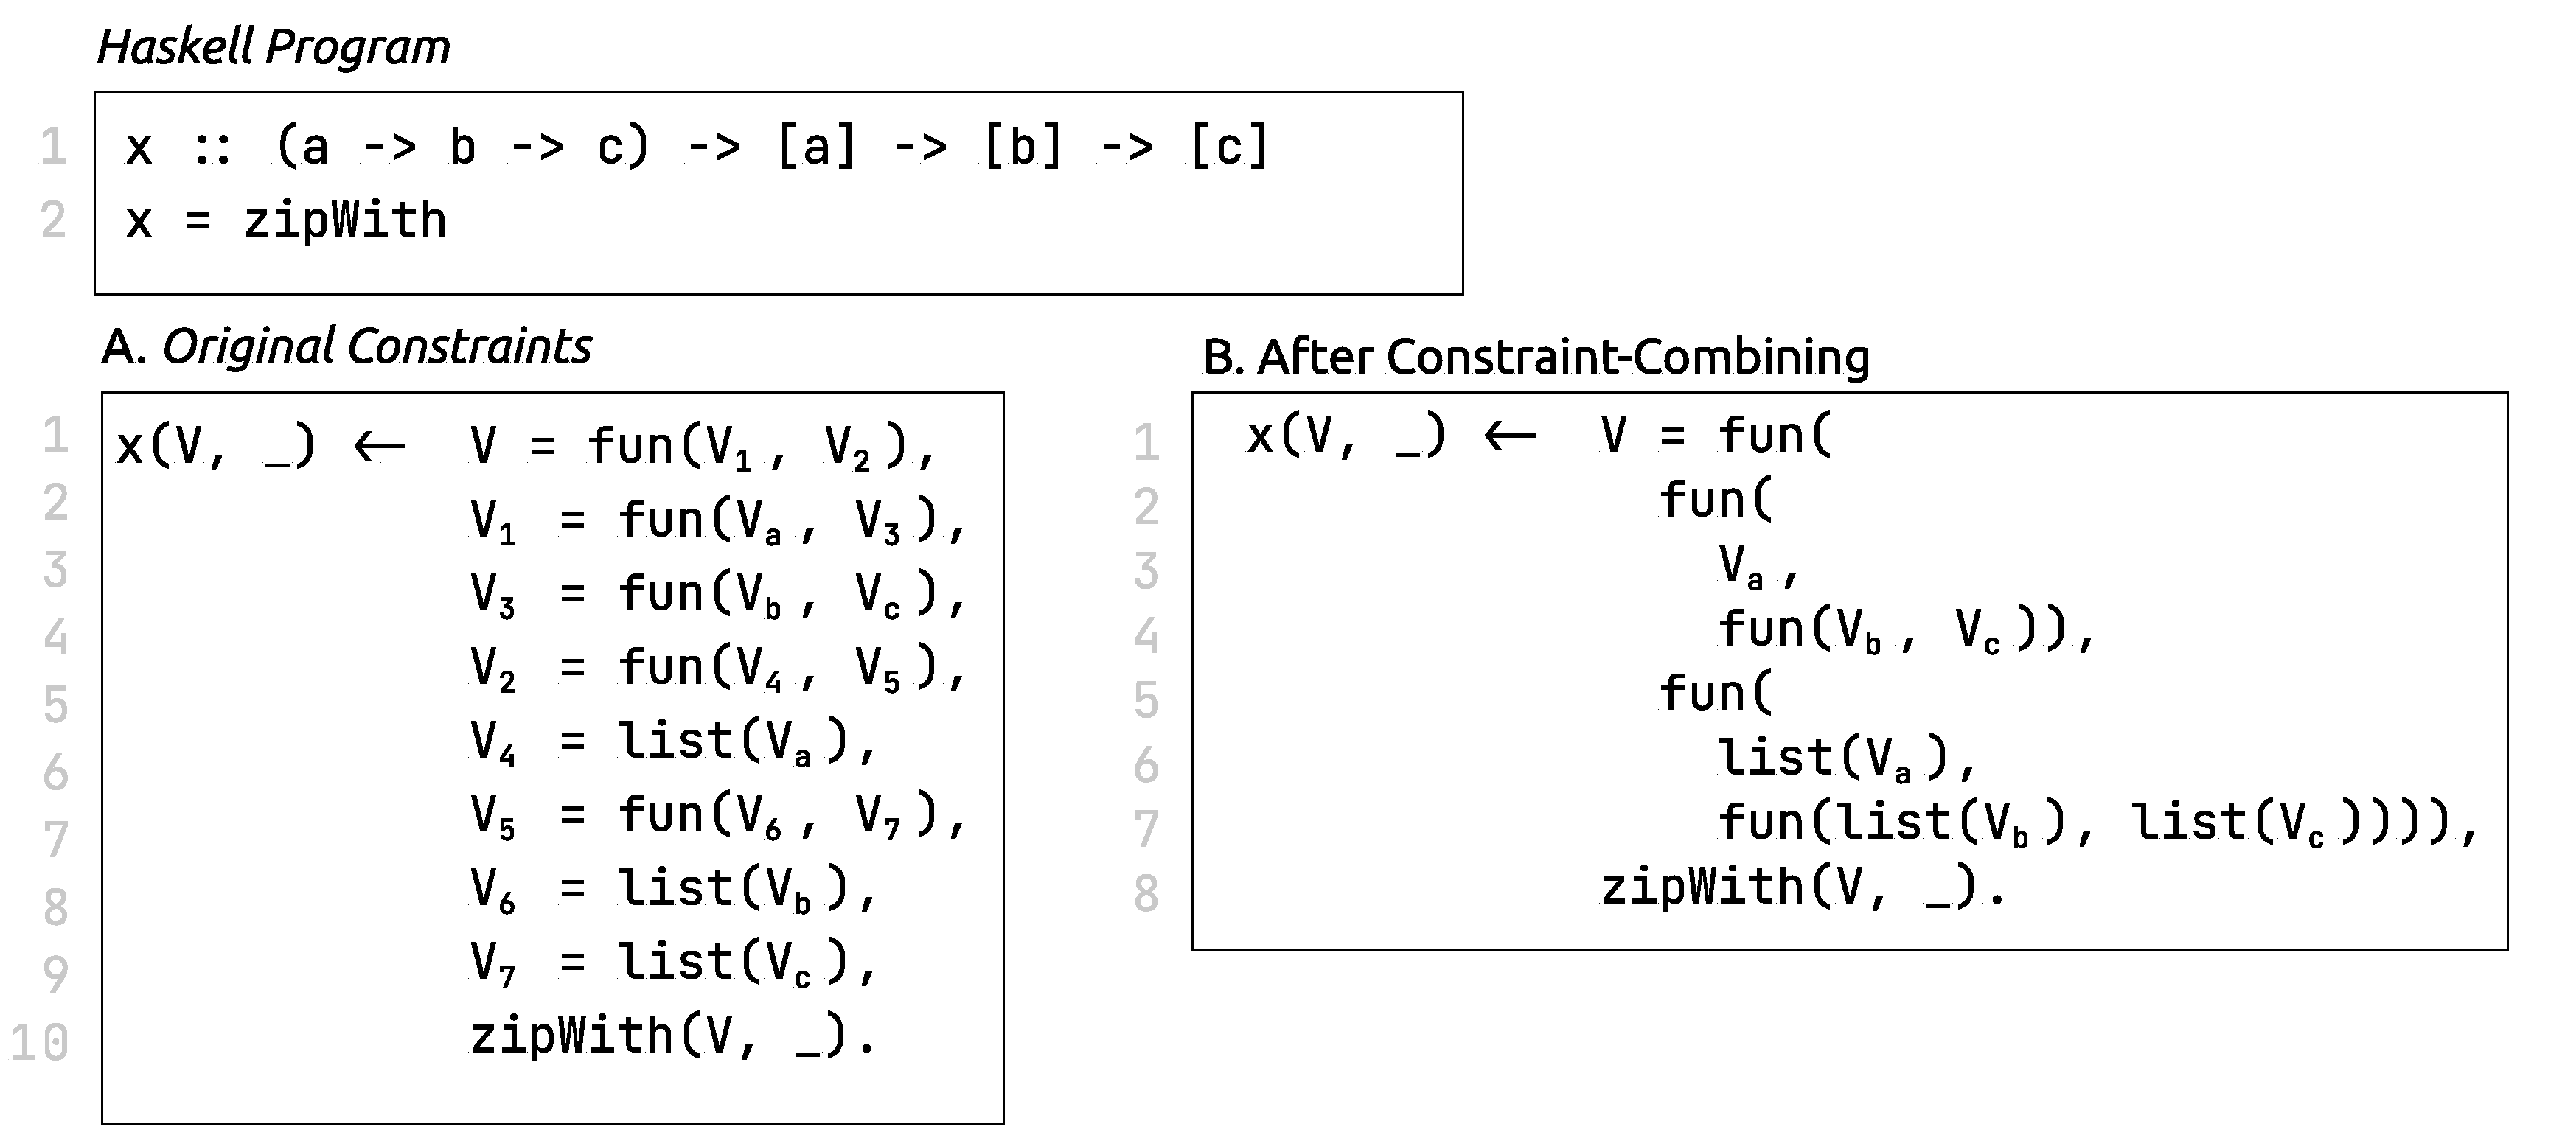
\includegraphics[width=\linewidth]{images/Combine-Constraints}
        \caption[Combine constraints in type signature]{\textbf{Combine constraints in type signature.} For a simple Haskell program (top),  without any optimization, Goanna generates 10 constraints (bottom left), indicated by 10 subgoals in the predicate. By combining the constraints in the type signature, Goanna produces 2 constraints (bottom right).}
        \label{fig:combine-constraints}
    \end{figure}

    Consider the example in Fig.~\ref{fig:combine-constraints}. Without optimization, this code would spawn 10 constraints. However, applying this optimization can achieve an equivalent outcome with merely 2 constraints. Notably, this optimization forfeits the capability to suggest fixes for sub-expressions within a type signature, a decision that warrants some consideration but, in our experience, often leads to clearer error localizations.

    \paragraph{Elimination of Over-Fitting Resolutions.}
    Over-fitting often refers to a situation where error correction tools provide solutions that are technically correct but involve making unnecessary modifications. In Goanna, every syntax node in the source code generates one or more constraints. This includes structural nodes such as function applications and let expressions. However, very often, suggesting that the user should modify the entire function application expression is not particularly instructive when changing one of the arguments fixes the type error as well. Disabling suggestions for over-fitting solutions improves the clarity of the suggestion list and enhances the speed of MCS enumeration.
   

    \paragraph{Elimination of Redundant Causes.}
    Goanna iterates over the possible causes and removes the ones that fail to deliver new insights. If all locations in a cause suggestion have already been covered in preceding suggestions, subsequent suggestions that merely rearrange these locations in different combinations can be omitted.
    
   \begin{figure}[ht!]
        \centering
        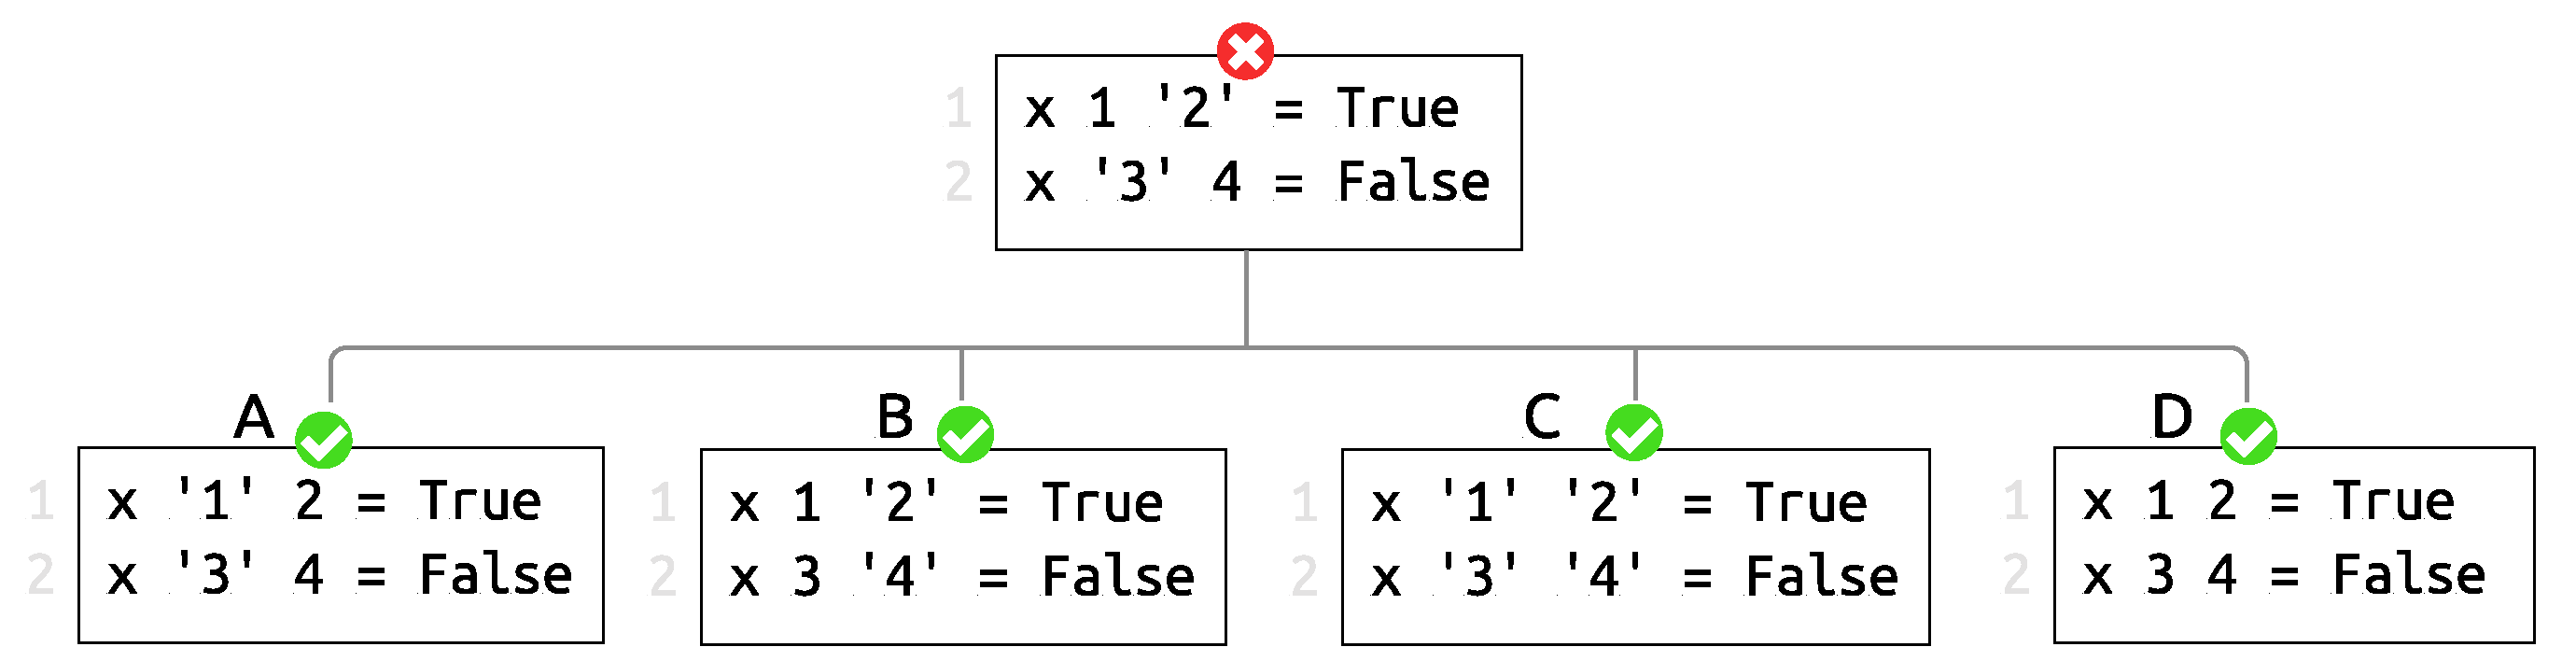
\includegraphics[width=0.9\linewidth]{images/Reduction-Example}
        \caption[The number of potential causes can grow exponentially]{\textbf{The number of potential causes can grow exponentially.} In the ill-typed Haskell program (Top), there are 4 different ways (Bottom) to fix the type error. It is not hard to see this growth is exponential, and showing all the alternatives is not helpful.}
        \label{fig:reduction-example}
    \end{figure}
    
    Consider the example in Fig.~\ref{fig:reduction-example}. Without knowing the true intention of the programmer, Goanna can provide four ways to fix the issue shown at the bottom. However, closer inspection reveals that after the first two suggestions, we no longer unearth new insights. Therefore, they can be removed to enhance the clarity of the suggestion list. 
    Note that this can remove the correct answer (say D), but if the programmer uses part of the (A) to make the fix, the revised type error will include the correct fix. 
    
    Removing superfluous MCS-based suggestions that recycle different permutations of the same set of locations is an instantiation of the Set Cover Problem (SCP). The problem can be rephrased as finding the minimal number of MCSes that cover all the potential locations that could cause the type error. Many approaches solve the SCP \cite{Caprara2000-vw}, including eager algorithms, linear programming, and heuristic-based algorithms. Generally, we found all of these approaches find the minimal cover of type errors efficiently. Goanna uses the OR-tools \cite{Google_Developers_undated-ew} for this task.
       
    \section{Evaluation} \label{sec:evaluation}
    The evaluation of Goanna focuses on some main it's ability to identify all error causes and rank them by their likelihood. Concretely, we want to answer the following key research questions about Goanna:

    Whether Goanna can identify type errors more accurately compare to traditional tools?
    How many potential fixes does Goanna provide for a typical type error?
    How fast does Goanna provide these type error diagnoses?
    
    \subsection{The dataset} \label{sub:dataset}   
    To assess Goanna, we extracted two datasets of defective Haskell programs. 
 The first (N=86), \texttt{Hakskell community},  from Haskell online discourse since 2018, each containing one or more type errors. The communities we searched include StackOverflow (32), Haskell on Reddit (20), and Haskell Discord Channel (34), as these are the top discussion channels for Haskell users according to research survey \cite{Fausak2022-zf}. During the search process, we looked for online discussions where the authors encountered type errors in their Haskell programs and asked for help. Further, we selected only the questions that had been answered and accepted by the original author.  We extracted the defective Haskell programs and the accepted answers as the Oracle solution. A second dataset (N=67), \textit{Haskell Academic}, is compiled from the known dataset of research projects that study Haskell errors. The length of these programs ranges from 1 liner to 64 lines of code (mean=20, median=20). These programs span a variety of subjects, including basic syntax (14 files), lists (28 files), tuples (5 files), algebraic data types (22 files), higher-order functions (17 files), monadic operations and do notation (9 files), type classes (6 files), and built-in/library functions (24 files). The distribution of themes generally aligns with the breakdown of the different causes of the type errors from Tirronen's study \cite{Tirronen2015-nr}.  
    
    \begin{table}
    \centering
    \begin{tabular}{|p{5cm}|c|c|c|} \hline 
         \textbf{Paper} & \textbf{Type} & \textbf{Tool} & \textbf{Programs} \\ \hline 
         \raggedright How Type Errors Were Fixed and What Students Did? & Empirical Study &  &  14 \\ \hline 
         \raggedright Helium: for learning Haskell & System/Tool & Helium & 7 \\ \hline 
         \raggedright Diagnosing Haskell Type Errors & System/Tool & SHErrLoc & 1 \\ \hline 
         \raggedright SHErrLoc: A Static Holistic Error Location & System/Tool & SHErrLoc & 1 \\ \hline 
         \raggedright Counter-Factual Typing for Debugging Type Errors & System/Tool & Counter-Factual Typing & 2 \\ \hline 
         \raggedright Understanding beginners' mistakes with Haskell & Empirical Study &  & 2 \\ \hline
         \raggedright Learning to blame: localizing novice type errors with data-driven diagnosis & System/Tool & Nate & 5 \\ \hline
         \raggedright Type Debugging with Counter-Factual Type Error Messages Using an Existing Type Checker &  &  & 1 \\ \hline
         \raggedright Improving Type Error Messages in OCaml &  &  & 5 \\ \hline
         \raggedright Type Error Slicing in Implicitly Typed Higher-Order Languages & System/Tool & Type Error Slicing & 1 \\ \hline
         \raggedright Getting into the Flow & System/Tool &  & 1 \\ \hline
         \raggedright Learning user friendly type-error messages & System/Tool & LearnHaskell & 3 \\ \hline
         \raggedright ChameleonIDE: Untangling Type Errors Through Interactive Visualization and Exploration & System/Tool & ChameleonIDE & 4 \\ \hline
         \raggedright Investigating Compilation Errors of Students Learning Haskell & Empirical Study &  & 5 \\ \hline
         \raggedright The Chameleon Type Debugger (Tool Demonstration) & System/Tool & Chameleon & 6 \\ \hline
         \raggedright Proofs about a folklore let-polymorphic type inference algorithm & System/Tool & Algorithm M & 2 \\ \hline
         \raggedright Interactive Type Debugging in Haskell & System/Tool & Chameleon & 2 \\ \hline
         \raggedright Exploiting diversity in type checkers for better error messages & System/Tool & Lazy typing & 1 \\ \hline
         \raggedright Improving Type Error Diagnosis & System/Tool &  & 3 \\ \hline
         \raggedright Searching for Type-Error Messages & System/Tool & SEMINAL &  1\\ \hline
         \raggedright Finding Minimum Type Error Sources & System/Tool & MaxSMT based tool & 1 \\ \hline
    \end{tabular}
    \caption{Caption}
    \label{tab:my_label}
\end{table}

\begin{table}
    \centering
    \begin{tabular}{|c|c|} \hline 
         \textbf{Source} & \textbf{Programs} \\ \hline 
         StackOverflow &  32 \\ \hline 
         Haskell on Reddit & 20 \\ \hline 
         Haskell Discord & 34 \\ \hline 
    \end{tabular}
    \caption{Caption}
    \label{tab:my_label}
\end{table}
 	\subsection{Accuracy and Reliability}\label{sub:eval-accuracy}

	Accuracy in type error diagnosis indicates whether the reported error match the user's real intention. Reliability measures how often can the type error be resolved user making any changes to the reported location. For each program, we compare Goanna's error diagnosis match the oracle answer. We consider the diagnosis accurate only if its suggested fix matches the accepted answer. We consider a diagnosis reliable when it can remove the type error if changes the reported location to a value of bottom type (undefined in Haskell).
  
  Goanna is compared with Glasgow Haskell Compiler (GHC) versioin 9.4 \cite{Gamari_undated-zu}, and Helium \cite{Hage2023-kk} version 1.8. GHC is the most widely used Haskell compiler, and it has established a reputation in the Haskell community for its wide capability, and great efficiency in working with Haskell projects. Helium is acknowledged for producing high-quality error messages \cite{Heeren2003-kd}. Because Goanna provides a comprehensive list of possible causes, while other tools only have one shot, therefore, we only include two variatino of Goanna: Goanna-1 (Only pick the top suggestions and discard all others) and Goanna-3 (Pick the top 3 suggestions and discard others).

  For all the errors in the dataset, there are no disagreements on the presence of errors among the 3 tools. In other words, Goanna did not miss any error that are caught by compiler tools. From the graph in Fig.~\ref{fig:accuracy}, GHC's accuracy is the least performant among all tools. Goanna 1's, although lower than Helium (72.1\%) in partial accuracy, is higher than Helium (51.2\%) when considering only diagnoses that fully match the accepted answer. \textbf{Goanna 3 has the best accuracy (84.8\%)}, higher than the partial accuracy of other tools. We carry on our disccuss on Goanna's accuracy with concrete examples in section \todo{ref}. 

  
     \begin{figure}[ht!]
        \centering
        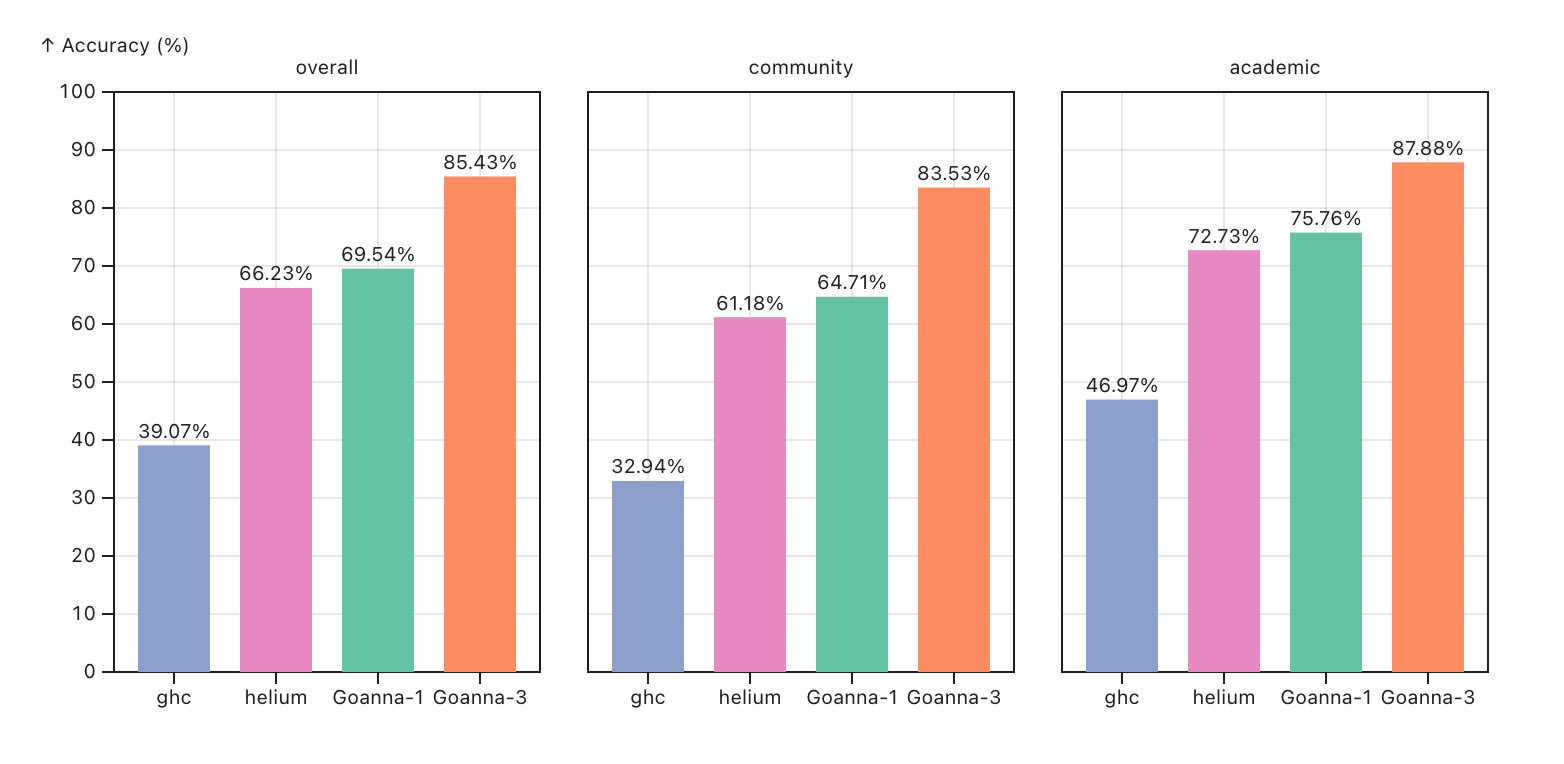
\includegraphics[width=\linewidth]{images/accuracy.png}
        \caption{The percentage of diagnoses that match the accepted answers.} 
        \label{fig:accuracy}
    \end{figure}

  \textbf{Reliability} shows similar patterns, in Fig. \ref{fig:reliability}, GHC is the least reliable (84.55\%) and Helium is about the (88.20\%) and Goanna-11 and Goanna-3 perform the same which is all (99.93\%). Some pattern that may surprizes reader is the reliability of Goanna-3 is less than Goanna-1. This is due to sometimes the 2nd and 3rd suggestions being included do not result in resolution. An example is \todo {show example}.

   \begin{figure}[ht!]
        \centering
        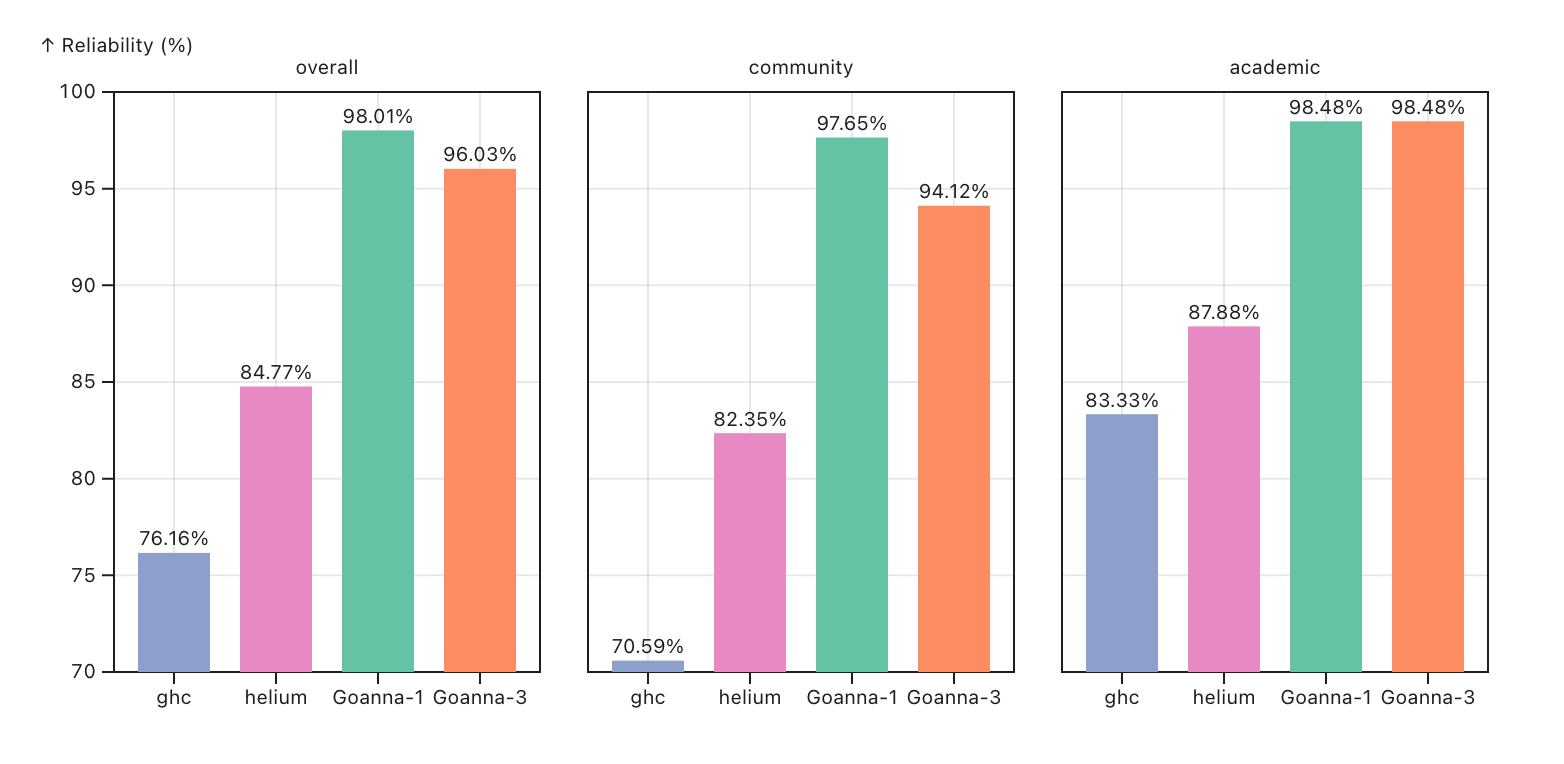
\includegraphics[width=\linewidth]{images/Reliability.png}
        \caption{The Reliability of Goanna} 
        \label{fig:reliability}
    \end{figure}


    % Because Goanna compute all the theoretically viable solutions to a type error, it is important for it to present the diagnosis in a way that promotes clarity. We consider to important aspect of clarity: reducing the number of potential causes to a small number, prioritise the potential causes that are more likely to be the root cause.  As we discussed in the previous section, Goanna uses a few such techniques to exclude nonsensicle or redundant causes, and Goanna also rank the causes by their likelyhood. We evaluate the clarity of gonna based on the number of total results provided by Goanna of each tasks. 

    % We compare compare the number of suspects identified by Goanna after and before the articulation process. And for the oracled cases, it is important to show that there are no cases where Goanna lost the true cause in the process of articulation.
    % \begin{figure}
    %     \centering
    %     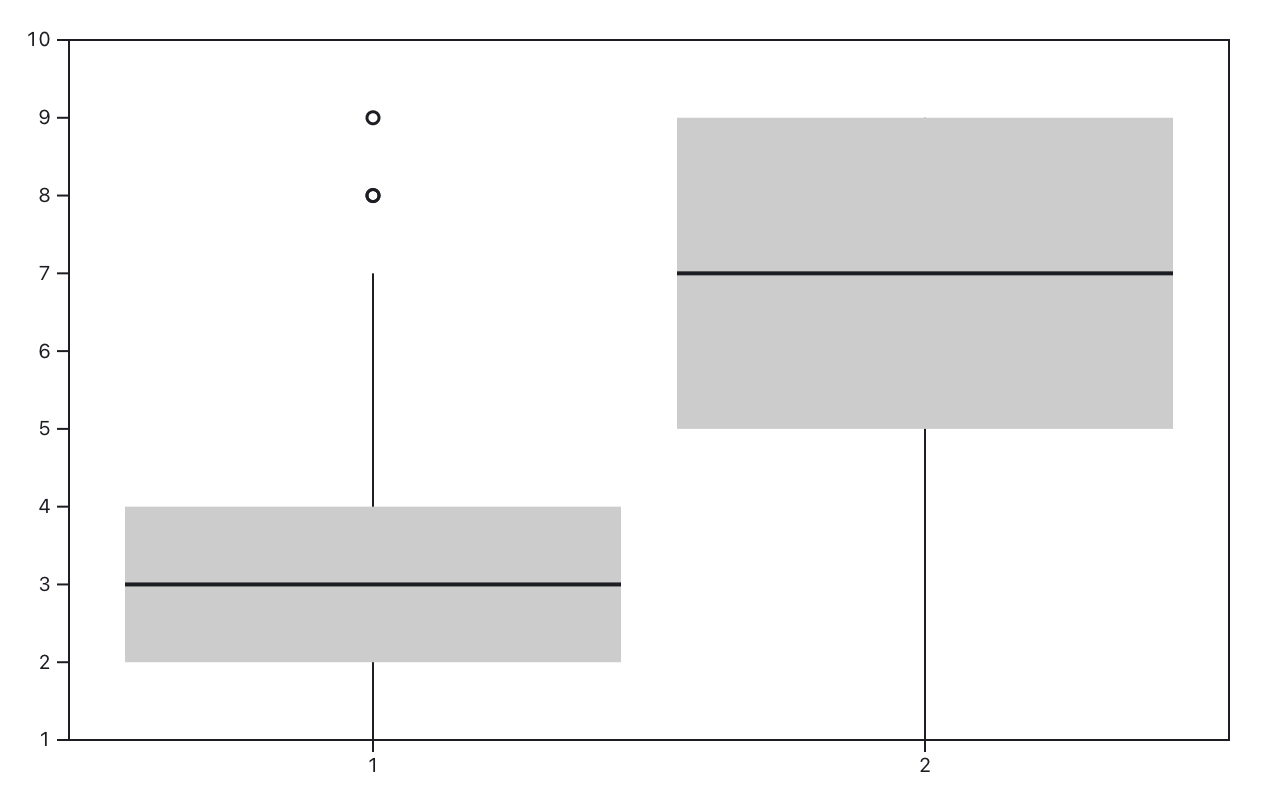
\includegraphics[width=0.5\linewidth]{images/CleanShot 2024-08-14 at 10.36.30@2x.png}
    %     \caption{Number of suspects identified by Goanna. }
    %     \label{fig:clarity}
    % \end{figure}

    % \begin{figure}
    %     \centering
    %     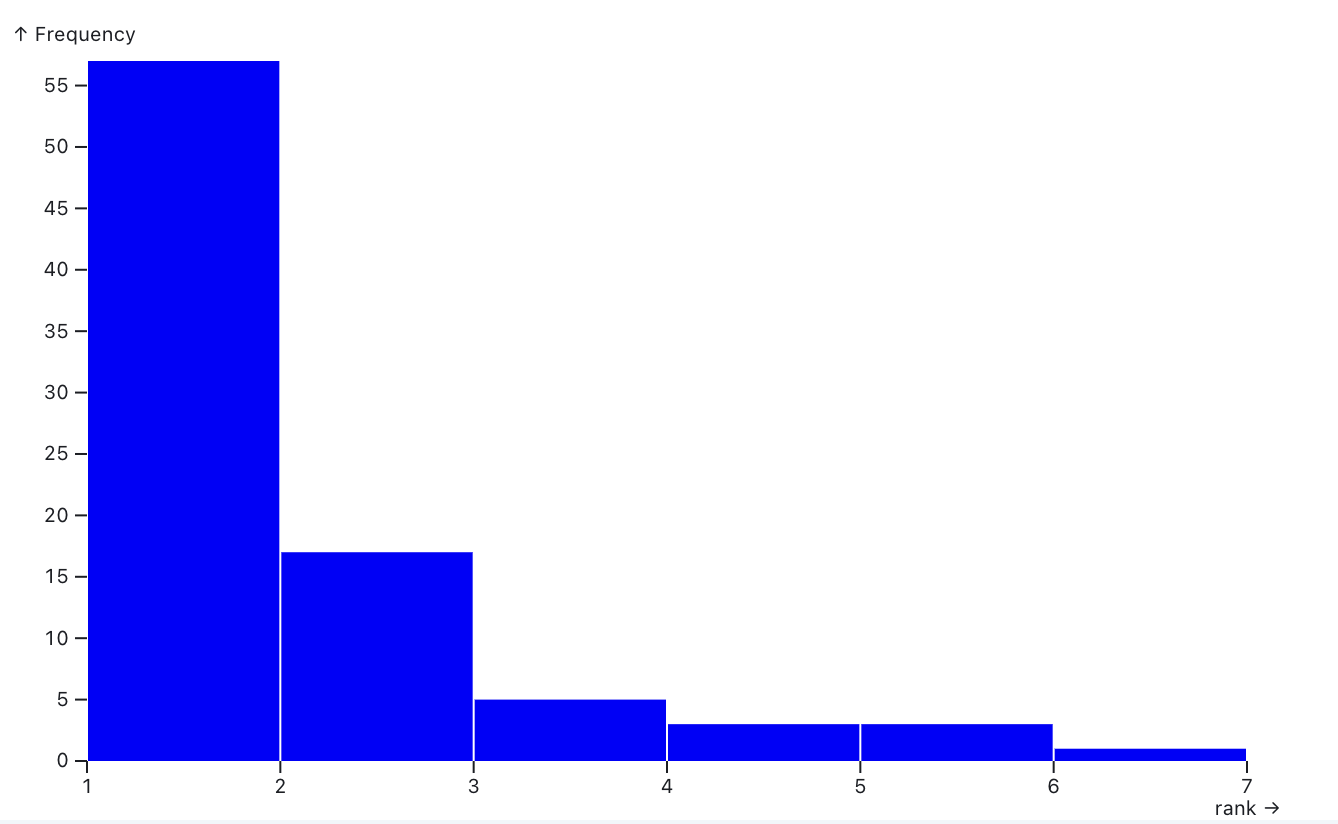
\includegraphics[width=0.5\linewidth]{CleanShot 2024-08-14 at 17.00.58@2x.png}
    %     \caption{Correct Answer Rank}
    %     \label{fig:correct-answer-rank}
    % \end{figure}

    \subsection{Performance} \label{sub:eval-performacne}
    First we show the time it takes for different tools to type checking the two dataset. Because Goanna does not terminate until all causes are detected and ranked, there is no point differenciating Goanna-1 and Goanna-3 as they perform idtentically. The result (Fig. \ref{fig:performance}) shows that Goanna performs slower than other tools. GHC (mean=0.09s, median=0.09s), Helium (mean=0.31s, median=0.31s) and Goanna (mean=0.50s, median=0.42s). In addition, Goanna has larger variation than other tools.

    To understand Goanna's performance in proper context, we use program synthetize to generate programs to precisely control a few important variables.  These include: the size of source program, what is the nature (category) of the type error, and the complexity of the type error (how many locations are involved overall).  We looked at the effect of complexity on multi-step type errors and multi-witness type errors, and how they differ. 


   \begin{figure}[ht!]
        \centering
        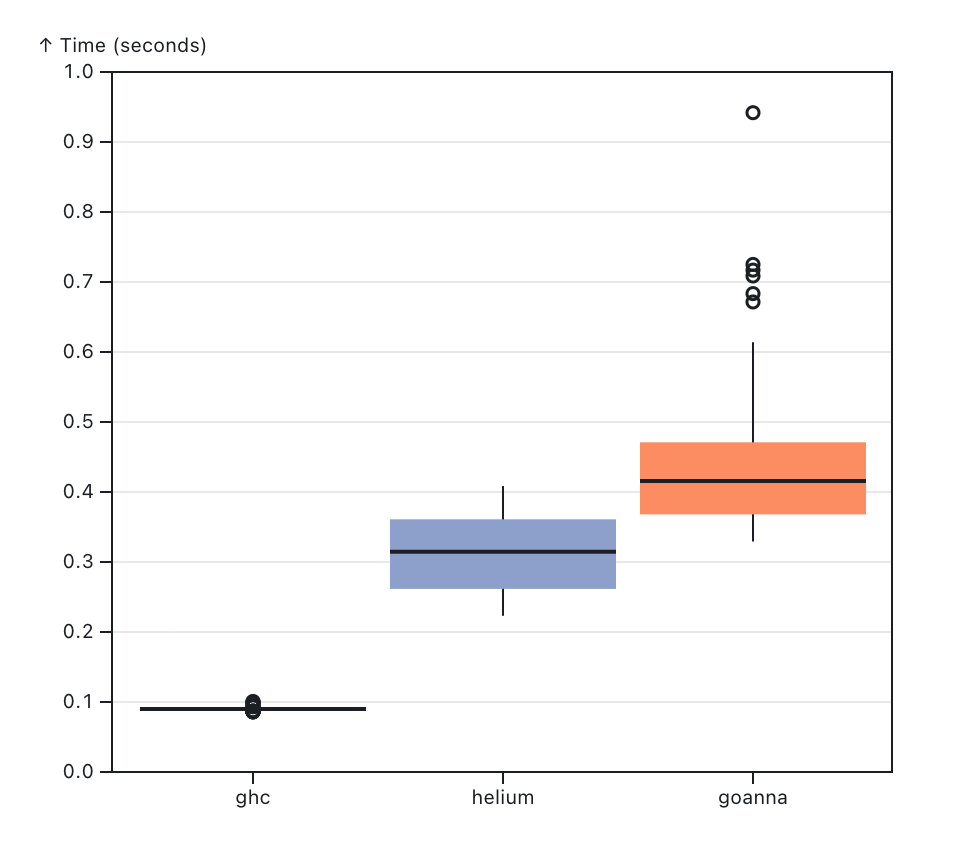
\includegraphics[width=0.7\linewidth]{images/performance-overall.png}
        \caption{Performance} 
        \label{fig:performance}
    \end{figure}
    
    The technique of generate defective program is showed in Fig. \ref{fig:error-generation}. To add complexity to a multi-step error, we simply add another step, usually a intermediate variable. To add complexity to a multi-witness error, we add a witness to a random side of the conflict. To add complexity to multi-party error, we add a new party. To simplify increase the program size without adding complexity, we add one or more well-typed top level declarations. We often need the last transformation to pad a program to be the same length as one with a more complex error.

    
    \begin{figure}
        \centering
        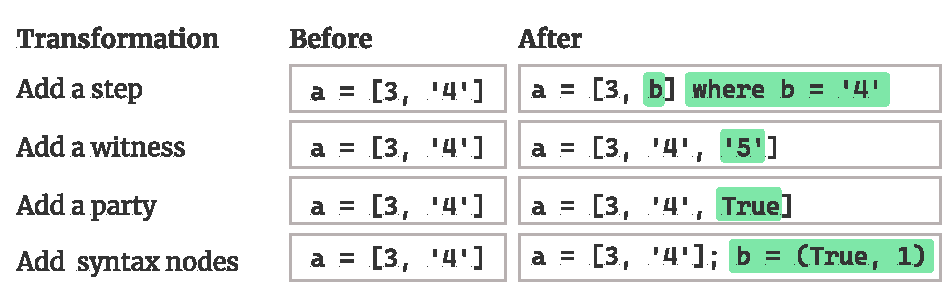
\includegraphics[width=0.5\linewidth]{images/evaluation-generating-errors.pdf}
        \caption{Enter Caption}
        \label{fig:error-generation}
    \end{figure}

    
    % We have to acknowledge that the speed is limited by the underlying technology used to enumerate the MUS, and more importantly the tools we used to verify whether the constraint system is satisfiable: the sat function. The general approach is to first reduce the amount of sat function calls, and second to speed up each sat function call. On the first approach, Goanna uses MARCO+ to reduce the sat function call. On the second approach, Goanna employs a few approaches to reduce the number of overall constraints.

    \paragraph{\textbf{The size of source program}}

    One important variable that affacts Goanna's performance is the size of source program. To measure this effect, we use generated program from 10 syntax nodes to 1200 syntax nodes. From Fig.~\ref{fig:node-size} we can see the size of program has profound effect on Goanna's ability to produce diagnosis. When a simple error with two potential fix locations, such as \texttt{x :: Int; x = 3}, and other declarations that are well-typed, it takes 0.25 seconds when there are 200 syntax nodes (roughly 20 lines of code), but it takes 7 seconds when there are 1200 syntax nodes (roughly 120 lines of code). Also can be seen from the graph is that more complex type errors (with more relevant locations) do affect the overall time of diagnosis. 

    \begin{figure}[ht]
        \centering
        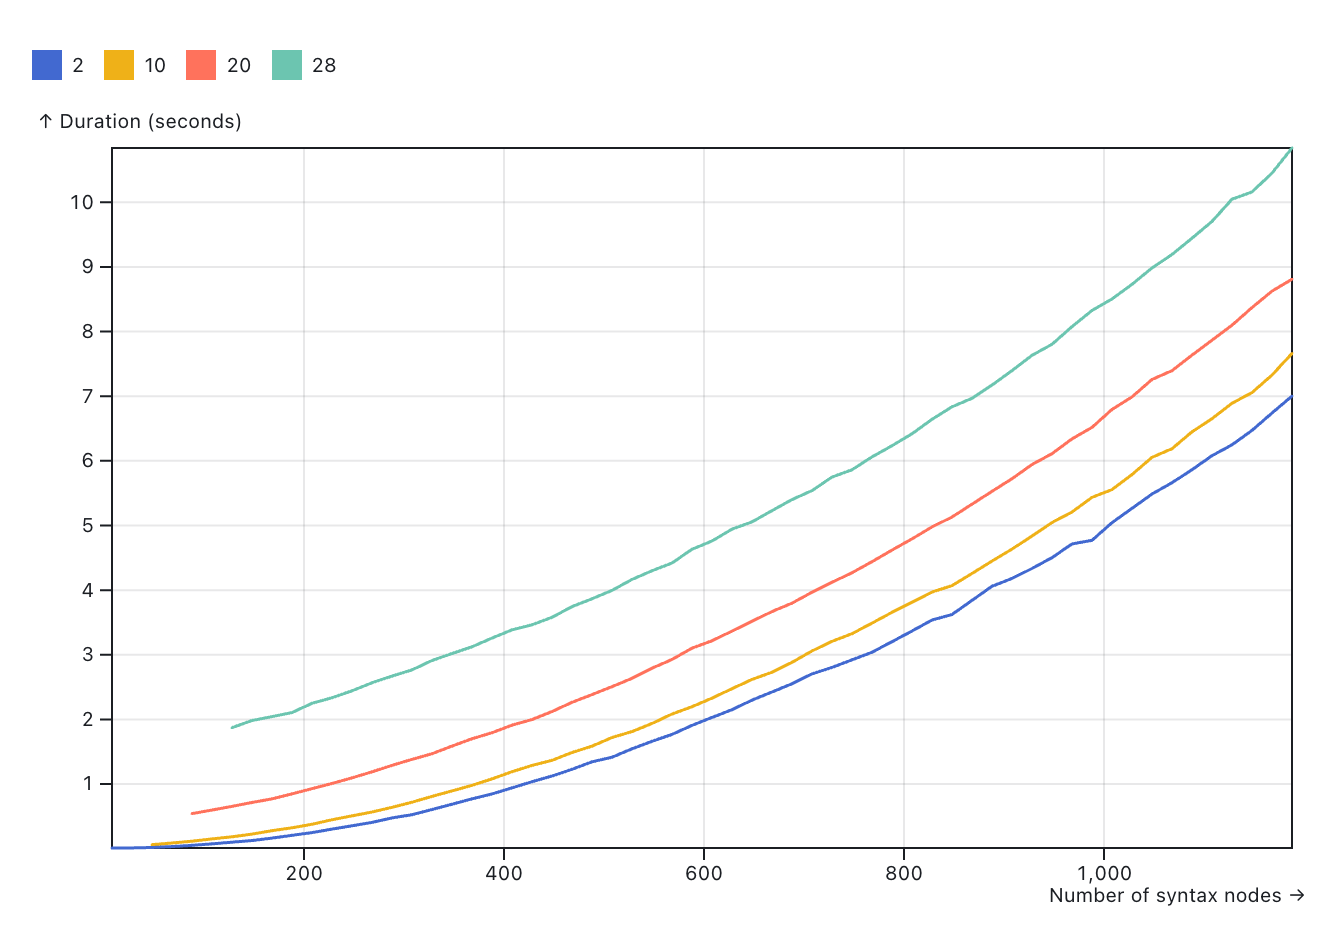
\includegraphics[width=0.8\linewidth]{images/program-size.png}
        \caption{Goanna's performance in relationship to different program sizes. The program size is measured in the number of syntax nodes.}
        \label{fig:node-size}
    \end{figure}

    To note, it may be tempted to think this correlation of performance and program size is due to the inefficiency of the parser and static analysis (such as gathering bindings and scopes). We show that the parser and static analysis is negligible even when the file grow to reasonably large and complex. The curprit here is the time it takes to enumerate the MUS and more precisely the number of MUSes. 

    % \paragraph{\textbf{The Time to First MUS output}}

    
    \paragraph{\textbf{Performance of Analyzing Multi-step Type Errors}}
   To understand how hard computationally taxing it is to finding all possible causes in a multi-step type error, we generate a series of defected programs that contains the same multi-step error but the number of steps keep increasing in the series from 2 to 30. In real world programming, encountering a Multi-step error with more than 10 step is rare. We also padded all programs to contain the same number of syntax nodes to remove the effect of program size. we generated programs containing multi-step type errors, for example, \texttt{x = 1; y = x; z = y; w = if True then z else '2'} has a step of 4. The result is shown in Fig. \ref{fig:multi-step-time}. For a program with 200 syntax nodes, it takes 0.275 seconds;  it takes 2.8 seconds when there are 30 steps. The same pattern can be found with programs with different numbers of syntax nodes. The pattern can be seen more readily in Fig \ref{fig:multi-step-cell}.
    
 \begin{figure}[ht]
        \centering
        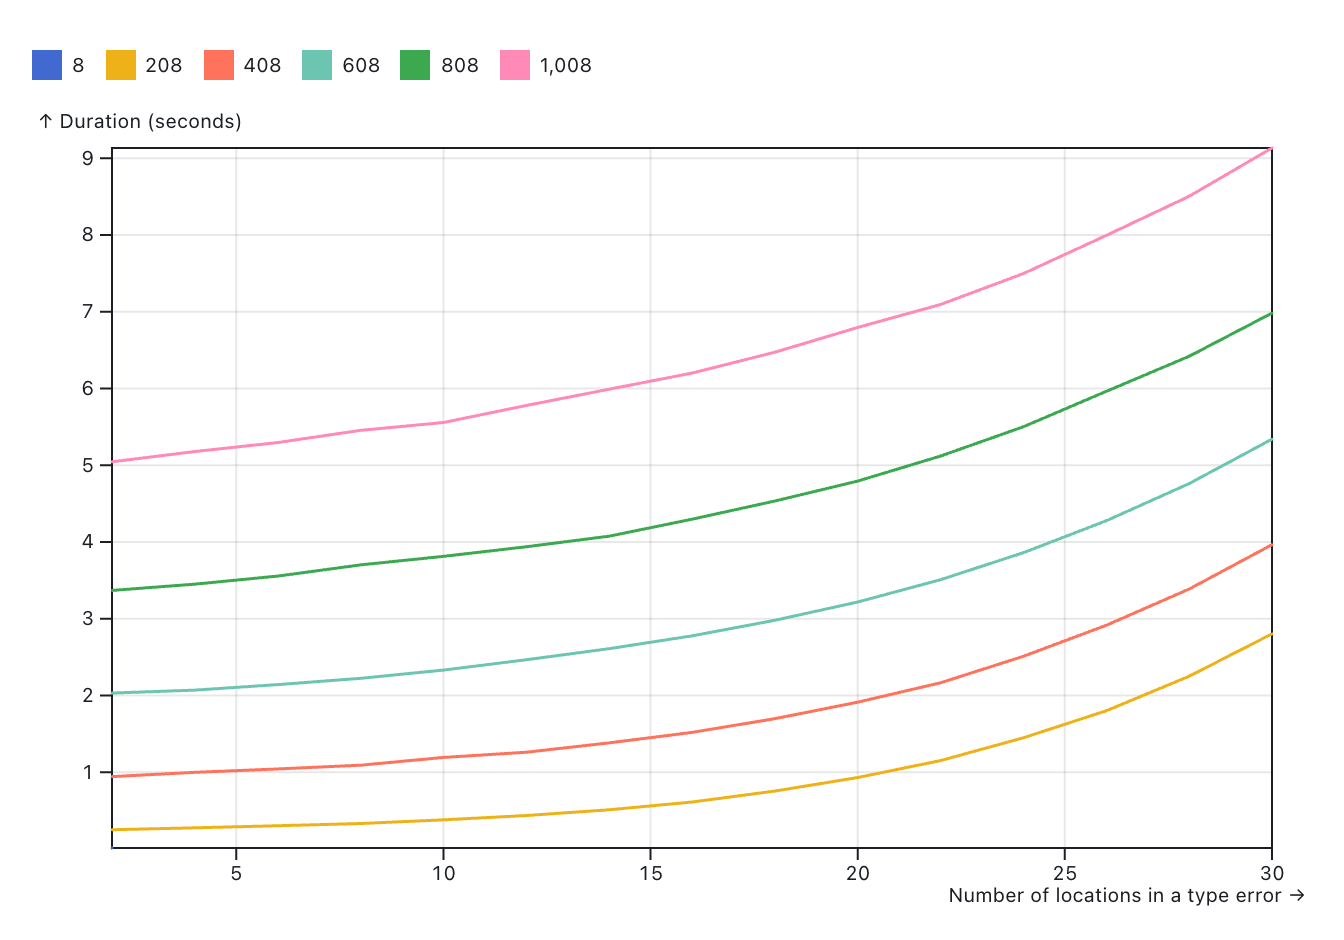
\includegraphics[width=0.8\linewidth]{images/multi-step.png}
        \caption{Goanna's performance in relationship to different program sizes. The program size is measured in the number of syntax nodes.}
        \label{fig:multi-step-time}
    \end{figure}


 \begin{figure}[ht]
        \centering
        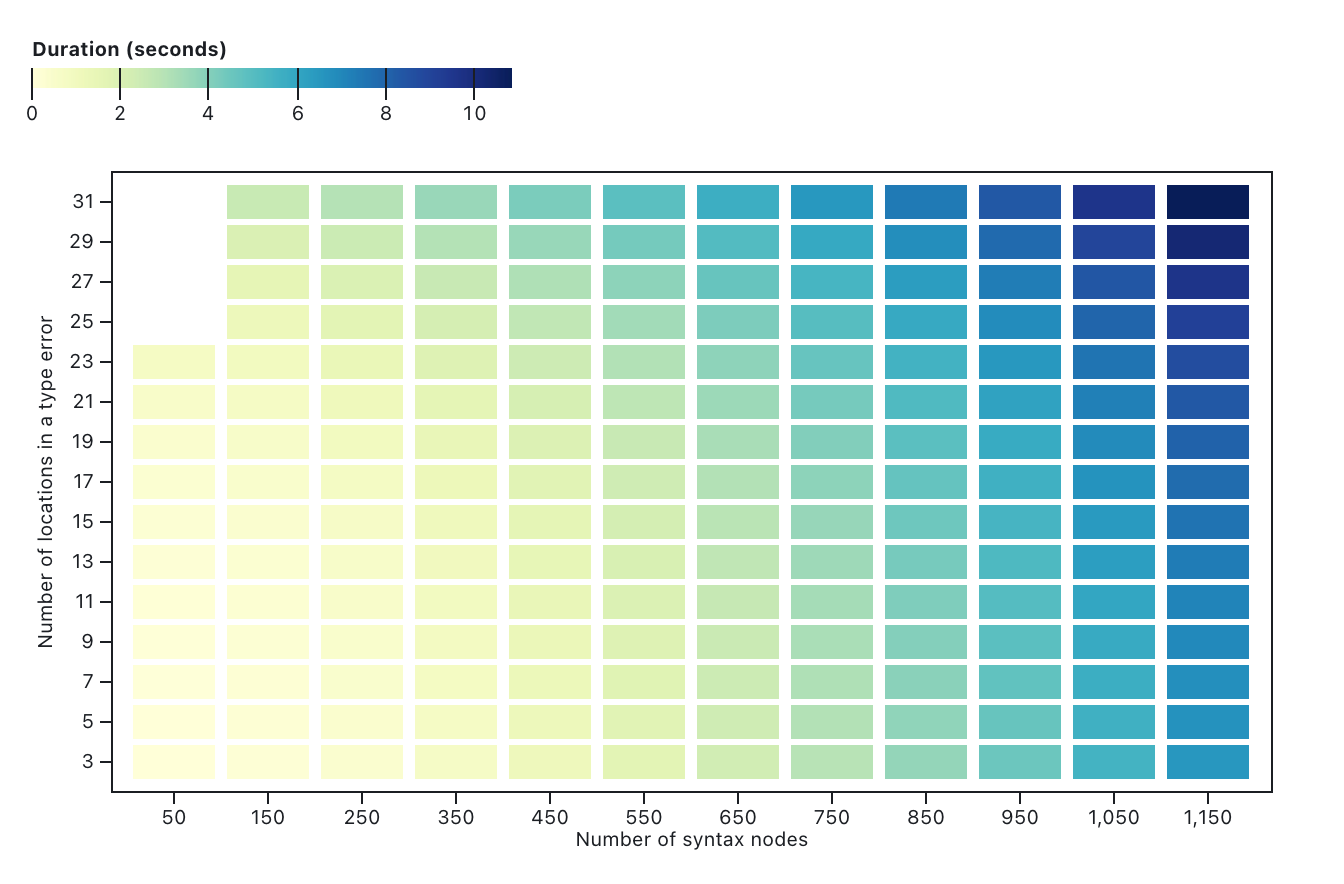
\includegraphics[width=0.8\linewidth]{images/multi-step-cell-map.png}
        \caption{Goanna's performance in relationship to different program sizes. The program size is measured in the number of syntax nodes.}
        \label{fig:multi-step-cell}
    \end{figure}

    \paragraph{\textbf{Performance of Analyzing Multi-witness Type Errors}}

    We generate a series of programs that contains the same, ever growing multi-witness error. From \texttt{x y = case y of 1 -> 1; '2' -> 2; '3' -> 3}. 
    It turns out analyzing multi-
    Multi-witness type errors are more slow to diagnose than multi-step errors. Intuitively, Goanna needs to go through the permutations to find out a specific grouping of constraints with their removal the whole program will type check. In Fig \ref{multi-witness-time} we see that it is linearly effect on the overall time. However, the time it takes is longer than multi-step errors with the same number of error locations. In a program with 30 error locations and 208 syntax nodes, it takes similar amount of time comparing to a multi-step error. However for a program with 1000 syntax nodes and 30 error locations, it takes over 43.68 seconds. 
 \begin{figure}[ht]
        \centering
        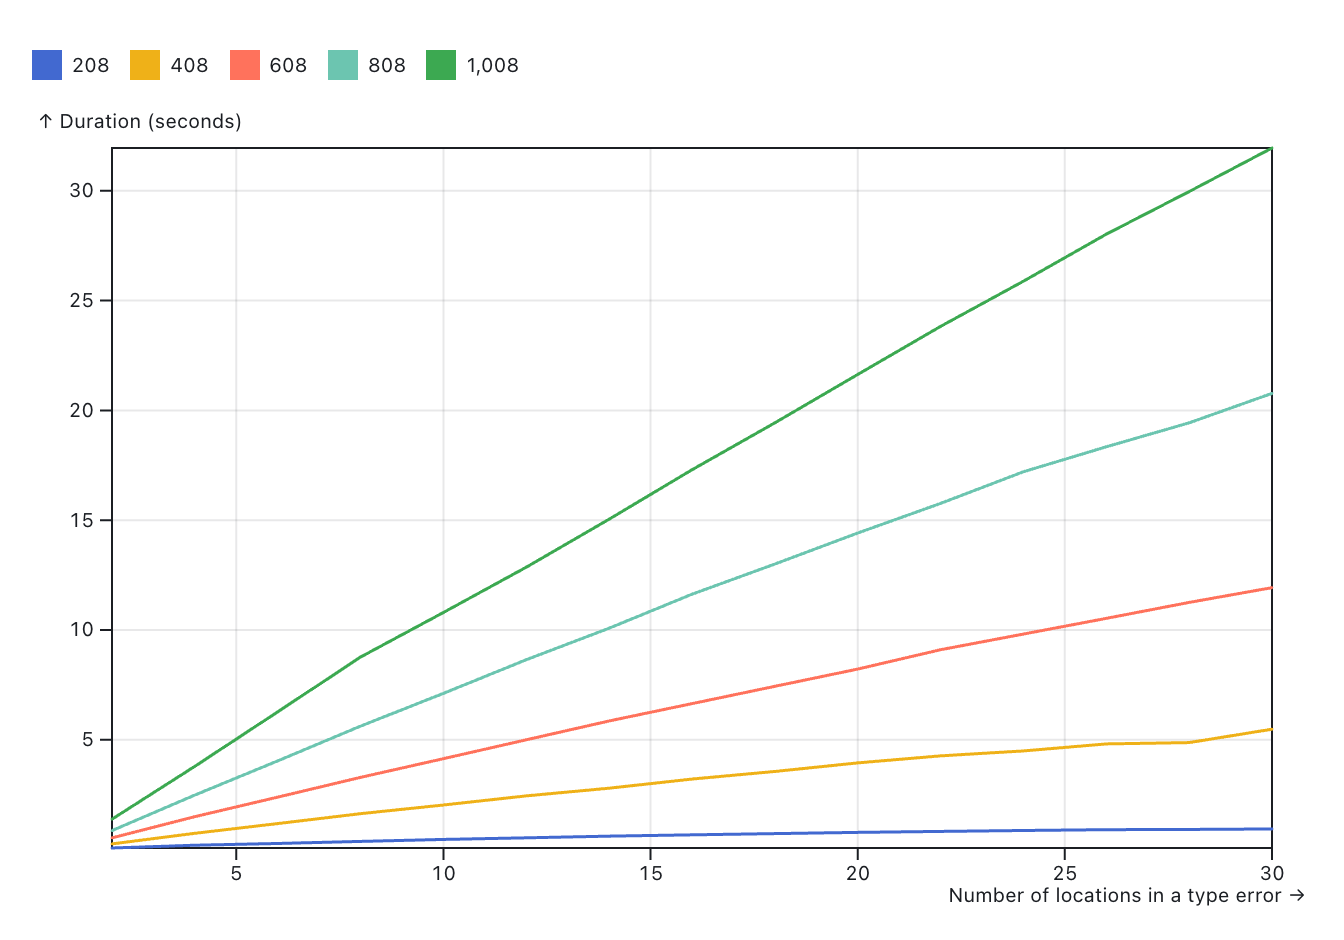
\includegraphics[width=0.8\linewidth]{images/multi-witness-time.png}
        \caption{Goanna's performance in relationship to different program sizes. The program size is measured in the number of syntax nodes.}
        \label{fig:multi-witness-time}
    \end{figure}
  
   \paragraph{\textbf{Performace of Analyzing Multi-party Type Errors}}
    Multi-party type errors are often more than one smaller type errors in disguise. For example, \texttt{x = [1, '2', "3"]} can be seen as two simple type errors combined into one. No matter which one programer fixes, the other one remains. To generate multi-party type error, we start with a base defect similar to the example in Listing \ref{lst:eval-multi-party} has a party of 3. We gradually increase the number of parties in the series of source programs to a 30 parties. The overall results is shown in Fig. \ref{fig:multi-party-time}. Multi-party errors are the most demanding category of all. For a program with 30 error locations and 200 syntax nodes takes 3.15 seconds. With 1000 syntax nodes, it takes 2 minutes and 34 seconds. To note, in real world programming, it is highly unlikely to encounter a multi-party type error with more than single digit, as programmer tend to deviate from well-typed state and quickly being resolved. 

\begin{lstlisting}[language=Haskell, caption=Multi-Party Hakslel Example, label={lst:eval-multi-party}]
data X = X
data Y = Y
data Z = Z
f a = case a of 
  X -> 1
  Y -> 2
  Z -> 3
\end{lstlisting}

 \begin{figure}[ht]
        \centering
        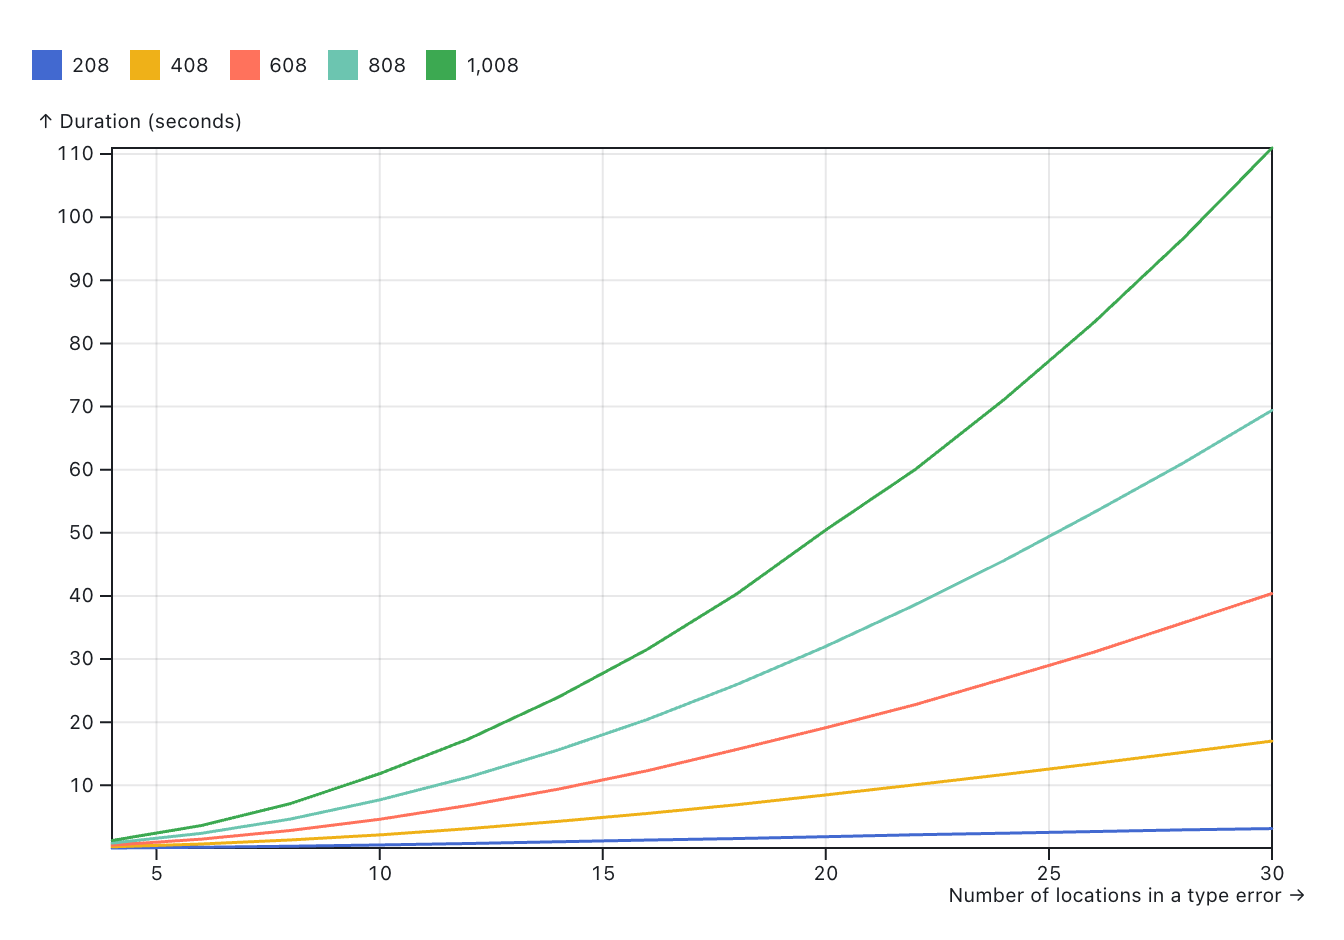
\includegraphics[width=0.8\linewidth]{images/multi-party-time.png}
        \caption{Goanna's performance in relationship to different program sizes. The program size is measured in the number of syntax nodes.}
        \label{fig:multi-party-time}
    \end{figure}

It can be clearly seen when put the 3 categories of type errors together, that multi-party type error is more demanding than other types, and multi-step type errors are the least demanding. 
     \begin{figure}[ht]
        \centering
        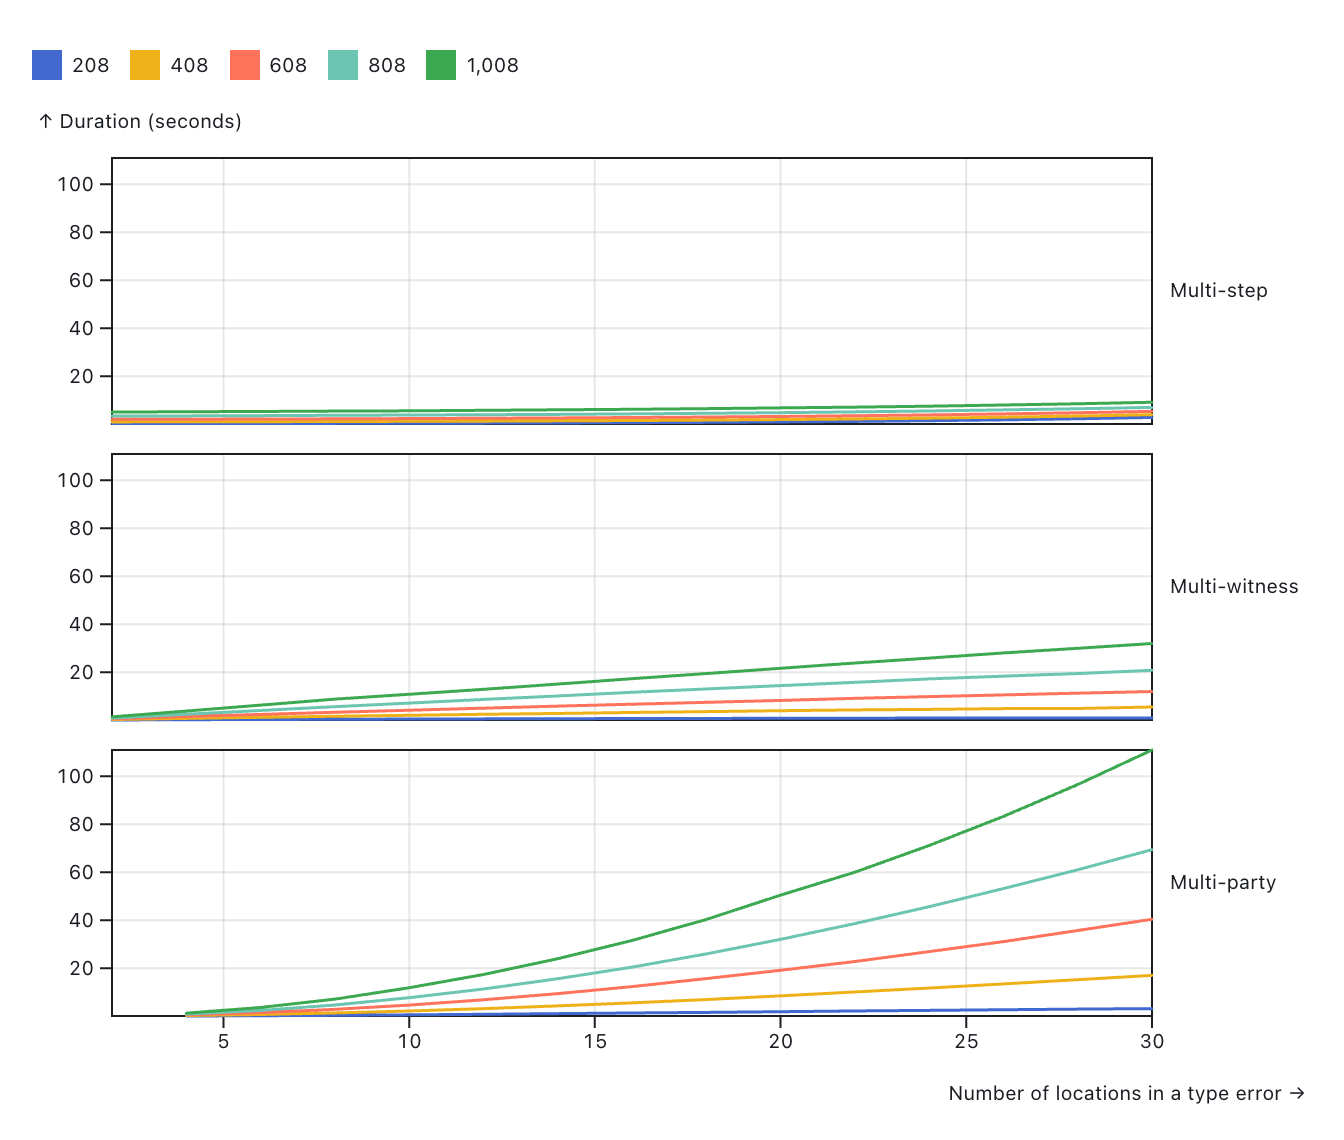
\includegraphics[width=\linewidth]{images/compare-time.png}
        \caption{Goanna's performance in relationship to different program sizes. The program size is measured in the number of syntax nodes.}
        \label{fig:compare-time}
    \end{figure}

    % \subsection{Threats to Validity}

    % \paragraph{\textbf{Selection of the dataset}}
    % Our selection of dataset is limited in its number. This is due to the challenge of finding programs that contain type errors. Unlike runtime errors, which can be mined from code repositories and version control histories, type errors in Haskell can be detected by the compiler tool, and ill-typed programs are usually fixed before the changes are committed to the version control systems. Further, we employed two selection methods. First, the error is indeed a type error. We test this by running the original program in GHC and checking if it indeed triggers a type error. The program is discarded otherwise, for instance, if it contains only parsing errors or runtime errors. Second, we discarded type questions where the main error relies on third-party libraries. 
    
  
        
    % \paragraph{\textbf{Measurement of performance}} Performance on Goanna and GHC was measured on a Linux virtual machine with a 3.1 GHz Processor and 2GB RAM. In practice, complex systems like this may perform differently depending on hardware and software configurations. Although we were not able to extract the performance profile of each tool across different platforms and operating systems, we chose hardware with abundant resources and up-to-date software dependencies. During our performance measuring, neither CPU usage nor memory usage was fully stressed. Additionally, GHC was run with the ``-fno-code'' flag enabled to limit its usage to type-check only.


    \section{Discussion} \label{sec:discussion}
    

    \subsection{Strengths of MCS-based error dignositcs}
    Traditionally MUS has been the go-to for modeling type error in a constraint satisfactory interpretation. Tools and studies include \todo{cite this}.

    MUS is good representation of type error because every MUS provide a complete chain of reasoning. This provide good indication on the location of the type error and the reason a conflict is detected. And often having one MUS is enough.

    Goanna is the first type debugging tool to use MCS and MUS. Comparing to MUS based approach, MCS provide more succinct cause analysis, meaningful ways to better guess the root cause, able to identify all type errors in the source file instead of just one, is able to infer the most concrete types for the entire source program with each potential cause.
    
    \paragraph{Unbiased Type Error}
    Unlike traditional compiler and type checkers such as GHC and helium, Goanna is not affected by left bias where only usage of a function is reported not the definition. Goanna does not stop when the first sign of a type error is encountered, instead collecting all the constraints and solve them wholesticaly, colliqually known as the french methdod. Goanna find all potentail causes and making it very easy for programmers to be review them one by one.
    This largely contribute to that Goanna outperfrom traditional tools in accuracy.
    
    In some cases, seeing how a type error can be fixed though other ways, even though not align with programmers' intention, is helpful for understanding the problem. 


    \paragraph{Meaningful and Familiar Idioms for Type error}
    MCS means the smallest change that will guide the user back to a well-behaved path of action. This type of error dignositics has been pracised in various places of user interface design such as autocrorrect software and git confilict resolution. Similarly, Goanna provides alternative solutions in a juxpositioned view. Programmers can review each one and see where are the changes going to be made and what are the effect of these changes in terms of typing.

    % A set of location mapped from MCS can be understood as the minimal amount of locations in the source code that needs to be modified to resolve the error state. This concept is well understood and offers clear insight into how the error occurs. In comparison, the traditional compiler tool, fails and report the last expression participated in the type checking, offers the interpretation: the type checking process was fine up to this step. Essentially, it means the reported location is guaranteed to be at least part of an suspected cause of the error. MUS based tool, like Chameleon, offers an interpretation: No matter how the error is caused, at least some part of the reported locations must another meaning: the reported location is a complete set of location of a potential cause of the error, but it may not be the true cause. I will illustrate how even choosing the wrong suspect can still lead to useful insight into finding the true cause.  

    % x = ['a', "b", 1]
    
    \paragraph{Full Type Hints on ill-typed Program}
    For implicitly typed languages, it is often beneficial to know the types of various expressions in the programs. Traditionally, these tools operate in interactive shells and command lines, such as \texttt{:t expression} in GHCI. Modern editors provide text overlay to support instant overview of these types. However, these type hints are only available when the program is well-typed, they either disappear or become outdated when type error occurs, where this kind of supporting information is most needed.

    Goanna is able to solve this issue by inferring types of all the surrounding expressions using MSS. MSS is the maximal set of constraints that represent a well typed portion of the source code, therefore concrete types can be assign to other part of the source code. Program can choose to ignore the type error for the moment and work on the rest of the program while enjoying the benefit of type hints.

    In addition, Goanna's type hints integrate with the idea of multiple causes, that is, the types of surrounding expressions changes when a different assumptions are made about the type error. So the type hints of Goanna is dynamic based on which cause is selected by the programmer.



 
 %    \subsubsection{MCS offers higher code reduction}
 %    In more complex tasks, MCS based type error diagnostic offer better code reduction than MUS based approaches. 
 % MUS-based error slicing can effectively eliminate program locations that are not contributing to a type error. However, research indicates that program slicing can effectively reduce only around 30\% of the code size that is required to understand a type error \cite{binkley_empirical_2007}. Further reduction is challenging with the knowledge of MUS alone due to the MUS's minimality. There are two contributors to why MCS approaches produce higher code reduction that MUS approach. First, source code are most of the time stay in they well typed state and occasionally diverge to a ill-typed state. Second, MUS representation of an error must include the intermediate `linking steps' which are common sense facts of the program. However these are hard to eliminated because excluding them the remaining constraints become satisfiable again, thus defeating the whole premise.   


 %    \subsubsection{Minimal Lossage Type Recovery enabled by MSS-based} 

 %    To assist the diagnostic of MCS-based error diagnosistic

    
    
    \subsection{Optimising Performance}
    Syntactic approach is to instead of using the constraints from the entire file, we divide it into top-level definitions and solve them sequencially in topological order. This has always been the way of how compiler tools type check gigantic projects. The downside is doing so we no longer use the  wholestic approach.

    A major challenge of MCS-based type dignositics is making it performant. As seen from our evaluation that it can be slower compared to state-of-art type checking tools. There are multiple avenues to address this issue: partiall
   Several approaches to achieve higher performance of Goanna show promise. The parallel capability of state of the art MUS enumeration \cite{Zhao2016-bu} algorithms are not explored in this study. With proper implementation, it will be possible to lower the hardware barrier of entry for wide adoption of MCS-based type error suggestion tools. Further, with domain-agnostic MUS enumeration tools \cite{Bendik2020-pz}, it should be possible to consistently achieve high performance while using a more performant constraint system and proper parameterization. Lastly, in a real-world implementation, it is possible to employ partial MUS enumeration \cite{Previti2013-mr,Liffiton2016-xi} to restrict the enumeration process in a sensible time-bound.

\subsection{Comparison with Large Language Models}
    
Our auto-calibration algorithm benefit from the observation that: in real life, almost all errors have multi-step. Humans are not easily fooled by ground level truths. Type conflict in literal level (e.g. \texttt{['2', "3", True]}) can be identified without tool assistance. However type conflict with multiple levels of interaction (e.g. \texttt{[x, y, z] where x = chr 65, y = '3':[], z = null y} are harder. Our auto-calibration algorithm simplifies these indirections when they start to introduce generate too many options. 

For multiple-witness type error generally do not increase the number of suspects. For multiple-party type errors, we observe that the number of type error is a factor of both the number of step and the number of parties. So in most of the cases, simply start to reduce the number of indirections can reduce the number of suspects of multiple-witness type error.


\section{Future Work}\label{sec:future-work}
\paragraph{\textbf{More Research Questions and Planned User Sudies}}
Can Goanna's accuracy
What user inter
It is important to evaluate Goanna with human participants and gain qualitative insight into its effectiveness. In one of our workshop preliminary studies, participants show positive reactions after using Goanna. A rigorous human study based on realistic debugging use cases is planned in the near future.   
  	
\paragraph{\textbf{Suggesting Syntax Approach}}
    One exciting path of improvement is to generate suggestions for syntax changes on top of type changes. As pointed out in \cite{Chen2014-dz}, syntax changes are much more challenging. But with the recent improvements of generative models and research advancement in ML-based type error \cite{Seidel2017-uf}, accurate syntax changes may be on the path to becoming feasible.

\paragraph{\textbf{Performance Optimization}}

\paragraph{\textbf{Supporting Other Languages}}
    Finally, it may be important to consider extending Goanna's capabilities to support other functional programming languages beyond Haskell. Several other languages, including Scala and OCaml, also support static typing and type inference, and Goanna could be a valuable addition in these contexts. In the future, we also hope to extend these techniques to popular multi-paradigm languages such as TypeScript and Rust.

  	
  	

    % Additional future work could include examining Goanna's integration with other tools within the Haskell development ecosystem. For instance, including Goanna in widely used text editors or development environments could offer a more integrated and fluid experience for developers and an important avenue for Goanna to reach a wider audience. 

    



\section{Summary} \label{sec:conclusion}
In this paper, we introduced Goanna, a tool for identifying and resolving type errors in Haskell code. We described the features of Goanna, including its fix suggestions, type error grouping, and identifying multiple type errors. We also discussed our approaches to reduce and reprioritize fix suggestions while maintaining comprehensiveness. Additionally, we walked through the uses of Goanna-IDE, a type error debugging interface for Haskell.

We evaluated the effectiveness of Goanna from a set of 86 diverse Haskell programs and demonstrated its ability to identify and resolve type errors accurately compared to other tools. We also showed that Goanna effectively condenses the list of causes. When a large number of causes is inevitable, Goanna's suggestion ranking heuristics ensures that more useful fixes are prioritized. Goanna currently works with Haskell, but in the future, we plan to extend its MCS-based error diagnosis to work with other strongly typed languages.
\bibliography{paperpile}

\end{document}
